\documentclass[en]{../../../eplsummary}

\usepackage{../../../eplcommon}
\usepackage{../../../eplcode}
\usepackage{wrapfig}
\usepackage{float}
\lstset{language=Java, basicstyle=\rm\small\ttfamily, tabsize=2}

\hypertitle[']{Algorithms and data structures}{5}{SINF}{1121}
{Antoine Paris, Sylvain Ramelot}
{Pierre Schauss}

% TODO
% - translate everything to english
% - improve a lot sections on basic data structures and sorting
% - add a subsection on trie in "Strings"
% - complete a bit subsection on data compression
% - add "Graphs" section

\section{Piles, files et listes chaînées}
\subsection{Listes chaînées}
\paragraph{Définition} Une \textit{liste chaînée}
est une structure de données récursive qui est soit
vide (\textit{null}) soit une référence vers un
noeud contenant une donnée générique et une référence
vers une liste chaînée.

Pour définir un noeud, on utilise une classe imbriquée :

\begin{lstlisting}
private class Node {
	private Item item;
	private Node next;
}
\end{lstlisting}

Une liste chaînée permet, si on possède un lien vers
le premier et le dernier élément de réaliser les
opérations suivantes en un temps indépendant de la
taille de la liste :

\begin{itemize}
	\item Insérer un élément au début ;
	\item Supprimer un élément au début ;
	\item Insérer un élément à la fin.
\end{itemize}

Pour pouvoir effectuer des insertions/suppressions
arbitraires efficacement, il faut utiliser des listes
doublement chaînées (chaque noeud possède deux liens,
un dans chaque direction).

Les implémentations de \lstinline{Stack}, \lstinline{Queue}
et \lstinline{Bag} reposent sur les listes chaînées. Grâce
à ces dernières, l'espace mémoire requis est proportionnel
au nombre d'items dans la collection et le temps requis
par opération est toujours indépendant de la taille de la
collection (ce ne serait pas le cas en utilisant des tableaux
par exemple).

\subsection{Stack}
Le principe de fonctionnement d'une stack est illustré à la figure
\ref{fig:stack}.

\begin{figure}[ht]
	\centering
	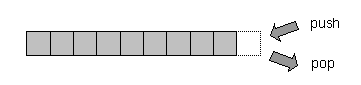
\includegraphics[scale=1.0]{img/stack.png}
	\caption{Illustration du fonctionnement d'une Stack LIFO.}
	\label{fig:stack}
\end{figure}

\lstinputlisting{code/Stack.java}

\subsection{Queue}
Le principe de fonctionnement d'une queue est illustré à la figure
\ref{fig:queue}.

\begin{figure}[ht]
	\centering
	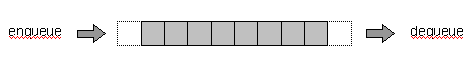
\includegraphics[scale=1.0]{img/queue.png}
	\caption{Illustration du fonctionnement d'une Queue FIFO.}
	\label{fig:queue}
\end{figure}

\lstinputlisting{code/Queue.java}

\subsection{Bag}
Un bag est simplement une stack sans méthode \lstinline{pop()}.

\section{Algorithmes de tri}
Le but du jeu ici est de trier des tableaux d'items contenant
chacun une clé en suivant un ordre bien particulier (le plus
souvent numérique ou alphabétique). La notion de clé est inclue
dans un mécanisme propre à Java, l'interface \lstinline{Comparable}
(et notamment la méthode \lstinline{compareTo}).

On distingue deux types d'algorithmes de tri, les algorithmes
\textbf{en place} qui n'utilisent pas (ou quasi pas) de mémoire
supplémentaire et ceux qui nécessitent assez de mémoire
supplémentaire pour garder une copie du tableau à trier en
mémoire.

Dans les algorthimes de tri présentés dans cette section,
on utilise le template suivant.

\lstinputlisting{code/SortTemplate.java}

\subsection{Selection Sort}
\subsubsection{Principe}
Le tri par sélection est un des plus simple. Il fonctionne
comme suit : premièrement, trouver l'élément le plus petit
du tableau et l'échanger avec le premier élément, ensuite
trouver le deuxième élément le plus petit du tableau et
l'échanger avec le deuxième élément, et ainsi de suite.
La traduction en Java est immédiate.

\subsubsection{Implémentation}
\lstinputlisting{code/Selection.java}

\subsubsection{Propriétés}
\paragraph{Le temps d'éxécution est indépendant de l'entrée}
L'algorithme mettra autant de temps à trier à tableau déjà
trié qu'un tableau aléatoirement ordonné.

\paragraph{Mouvement minimal}
Le nombre d'échange est une fonction linéaire de la taille
du tableau à trier ($N$ échanges sont effectués). 

\subsubsection{Complexité}
Dans tous les cas $\frac{N^2}{2}$ comparaisons et $N$ échanges.

\subsection{Insertion Sort}
\subsubsection{Principe}
C'est l'algorithme qu'on utilise en général pour trier
ses cartes. On considère une carte à la fois, et on
l'insère à sa place parmis les cartes déjà triées. La
seule différence est qu'ici il faut faire de la place
pour insérer l'item considéré à sa position, on doit
donc décaler tout les items plus grand que lui d'une
position vers la droite.

\subsubsection{Implémentation}
\lstinputlisting{code/Insertion.java}

\subsubsection{Propriétés}
Contrairement au tri par sélection, le temps d'éxécution
du tri par insertion est dépendant de l'entrée, il est par
exemple \textbf{excellent pour des tableaux presque triés}.

C'est également une méthode correcte pour de très petits
tableaux.

\subsubsection{Complexité}
Dans le pire cas, $\frac{N^2}{2}$ comparaisons et
$\frac{N^2}{2}$ échanges.

\subsection{Shell Sort}
\subsubsection{Principe}
Le shellsort est juste une simple extension du tri
par insertion. Dans le tri par insertion, les échanges
n'impliquent que des éléments adjacents, les items ne
peuvent donc se déplacer que d'un élément à la fois.
Le shellsort gagne en rapidité en autorisant des échanges
d'éléments éloignés dans le tableau.

\paragraph{Tableau $h$-trié} un tableau $h$-trié ($h$-sorted
array) est un tableau dont tous les éléments séparés
de $h$ positions sont triés.

\subsubsection{Implémentation}
Concrètement, l'algorithme s'implémente en utilisant le
tri par insertion pour obtenir successivement des 
tableaux $h$-triés avec $h$ décroissant.

\lstinputlisting{code/Shell.java}

\subsubsection{Propriétés}
Lorsqu'un tableau $h$-trié est $k$-trié, il reste
$h$-trié.

\subsubsection{Complexité}
Un peu moins quadratique, $N^{\frac{4}{3}}$, $N^{\frac{5}{4}}$
ou $N^{\frac{6}{5}}$ dans le pire cas.

\subsection{Mergesort}
Le principe du tri par fusion est assez simple : pour trier
un tableau, diviser le en deux moitiés, trier chaque moitié
(récursivement) et ensuite fusionner les résultats.

La complexité des algorithmes de tri par fusion est
logarithmique en $N\log N$. Le tri par fusion est
un algorithme de tri basé sur des comparaisons
asymptotiquement optimal (on ne peut pas faire mieux).

Les deux implémentations du tri par fusion vues ici
se base sur la méthode \lstinline{merge} suivante :

\lstinputlisting{code/mergeMethod.java}

\subsubsection{Top-down mergesort}
Ici, on divise le problème en sous-problèmes et on les résout
récursivement. 

\lstinputlisting{code/Merge.java}

\begin{figure}[ht]
	\centering
	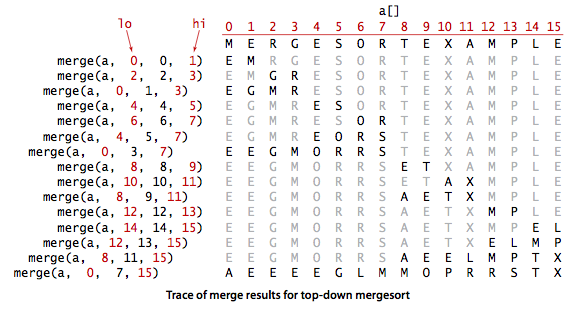
\includegraphics[scale=0.5]{img/mergesortTD.png}
	\caption{Trace des résultats de merge pour le top-down mergesort.}
\end{figure}

\subsubsection{Bottom-up mergesort}
Ici, on construit des petites solutions que l'on rassemble
pour en former des plus grandes à chaque fois. 

\lstinputlisting{code/MergeBU.java}

\begin{figure}[ht]
	\centering
	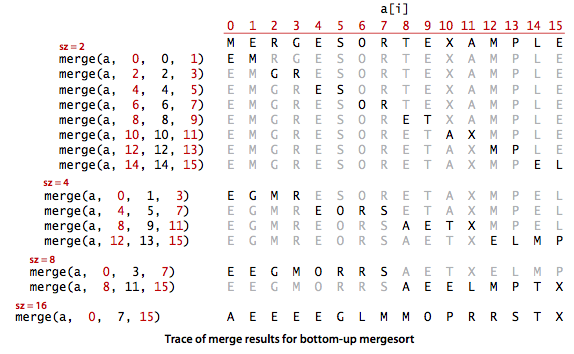
\includegraphics[scale=0.5]{img/mergesortBU.png}
	\caption{Trace des résultats de merge pour le bottom-up mergesort.}
\end{figure}

C'est la méthode à privilégier pour trier une liste chaînée.

\subsection{Quicksort}
\subsubsection{Principes}
Le tri rapide est probablement le plus utilisé, et ce pour
les deux raisons suivantes : il est en place et s'éxécute
en un temps proportionnel à $N \log N$.
Il fonctionne selon le principe du \textit{diviser pour
mieux régner}. Il partitionne le tableau en deux parties
et les trie ensuite indépendemment comme illustré sur
la figure \ref{fig:quicksort-overview}

\begin{figure}[ht]
	\centering
	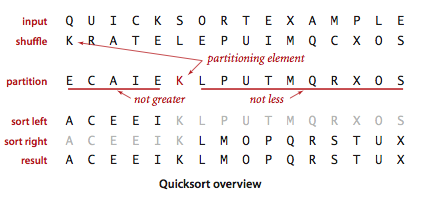
\includegraphics[scale=0.7]{img/quicksort-overview.png}
	\caption{Quicksort overview.}
	\label{fig:quicksort-overview}
\end{figure}

L'algorithme de partionnement doit réarranger le tableau pour que
les 3 conditions suivantes soient vérifiées :

\begin{itemize}
	\item L'entrée \lstinline{a[j]} est à sa position finale pour
	un certain $j$ ;
	\item Les entrées \lstinline{a[lo..j-1]} sont inférieures ou
	égales à \lstinline{a[j]} ;
	\item Les entrées \lstinline{a[j+1..hi]} sont supérieures ou
	égales à \lstinline{a[j]}.
\end{itemize}

Ces 3 conditions sont résumées sur la figure \ref{fig:part-overview}.

\begin{figure}[ht]
	\centering
	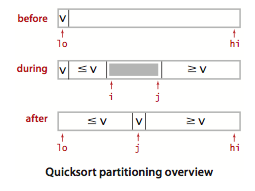
\includegraphics[scale=0.7]{img/partitioning-overview.png}
	\caption{Partioning overview.}
	\label{fig:part-overview}
\end{figure}

\subsubsection{Implémentation}
La trace du code suivant se trouve à la figure \ref{fig:part-trace}

\lstinputlisting{code/Quick.java}

\begin{figure}[ht]
	\centering
	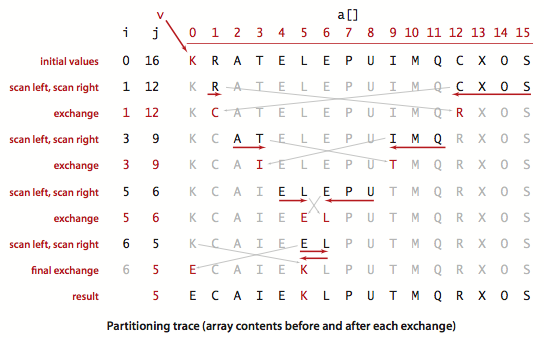
\includegraphics[scale=0.5]{img/partitioning.png}
	\caption{Partioning trace.}
	\label{fig:part-trace}
\end{figure}

\subsubsection{Complexité}
Dans le pire cas, le tri rapide a une complexité quadratique.
Il est possible d'éviter ce pire cas en mélangeant aléatoirement
le tableau avant de le trier (cela fait du tri rapide un
algorithme \textit{randomisé}).

Dans le cas moyen, le tri rapide a une complexité en $\mathcal{O}(n\log(n))$.

\subsection{3-way quick sort}
\subsubsection{Principes}
Si le tableau à trier contient beaucoup d'éléments dupliqués (voir \textit{Dutch
National Flag problem}), il est possible d'atteindre une complexité
linéaire en modifiant un peu le tri rapide.

L'idée est d'utiliser 3 partitions plutôt que 2, comme indiqué sur
la figure \ref{fig:part3-overview}.

\begin{figure}[ht]
	\centering
	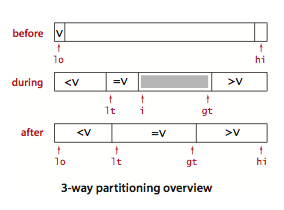
\includegraphics[scale=0.7]{img/partitioning3-overview.png}
	\caption{3-way partioning overview.}
	\label{fig:part3-overview}
\end{figure}

Pour cela, une solution est d'effectuer un simple scan de la gauche
vers la droite dans le tableau en maintenant une variable \lstinline{lt}
tel que \lstinline{a[lo..lt-1]} sont inférieurs à $v$, une variable
\lstinline{gt} tel quel \lstinline{a[gt+1..hi]} sont plus grands que $v$,
une variable $i$ tel que \lstinline{a[lt..i-1]} sont égals à $v$ et
\lstinline{a[i..gt]} n'ont pas encore été examinés.

% TODO : add summary of complexity for sorting algorithms

\subsubsection{Implémentation}
La trace du code suivant se trouve à la figure \ref{fig:part3-trace}

\lstinputlisting{code/Quick3way.java}

\begin{figure}[ht]
	\centering
	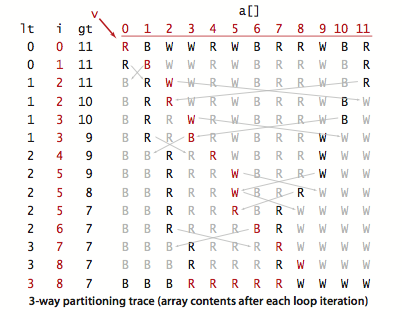
\includegraphics[scale=0.7]{img/partitioning3.png}
	\caption{3-way partioning trace.}
	\label{fig:part3-trace}
\end{figure}

\section{Searching}
\subsection{Symbol tables}
\begin{mydef}
A \textit{symbol table} is a data structure for key-value pairs that
supports two operations: \textit{insert} (put) a new pair into the
table and \textit{search} for (get) the value associated with a given
key.
\end{mydef}

Here we adopt the \textit{associative array abstraction}, where you can
think of a symbol table as being just like an array where keys are
indices and values are array entries.

The API for a generic basic symbol table is given in figure \ref{fig:st-api}.

\begin{figure}[ht]
	\centering
	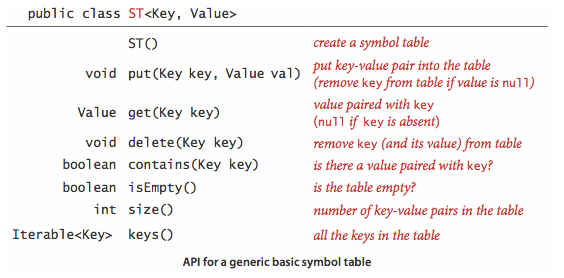
\includegraphics[scale=0.5]{img/symbol-table-api.png}
	\caption{API for a generic basic symbol table.}
	\label{fig:st-api}
\end{figure}

For applications where keys are \lstinline{Comparable}, we usually talk about
\textit{ordered symbol tables}, where keys are kept in order.

The API for a generic ordered symbol table is given in figure \ref{fig:ost-api}.

\begin{figure}[ht]
	\centering
	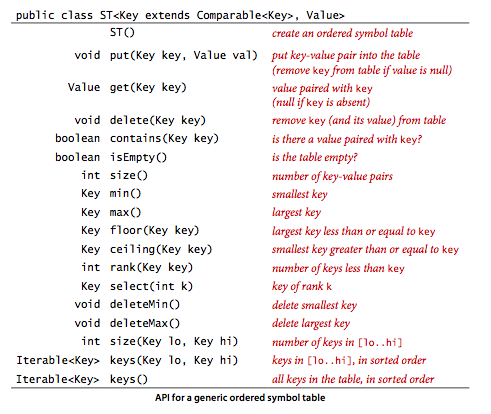
\includegraphics[scale=0.5]{img/ordered-symbol-table-api.png}
	\caption{API for a generic ordered symbol table.}
	\label{fig:ost-api}
\end{figure}

\subsubsection{Sequential search in an unordered linked list}
One straightforward option for the underlying data structure for a
symbol table is a linked list of nodes that contain keys and values.

Implementations of both \lstinline{get()} and \lstinline{put()} consist
of scanning through the list. Hence, it is easy to show that the worst
case is $\mathcal{O}(n)$ for both. In conclusion, a linked-list
implementation with sequential search is too slow to be used to solve
huge problems.

\subsubsection{Binary search in an ordered array}
\begin{lstlisting}
public class BinarySearchST<Key extends Comparable<Key>, Value>
{
\end{lstlisting}

Now, we consider a full implementation of our ordered symbol-table API.
The underlying data structure is a pair of parallel arrays, one for the
keys and one for the values.

\begin{lstlisting}
    public BinarySearchST(int capacity) { 
        keys = (Key[]) new Comparable[capacity]; 
        vals = (Value[]) new Object[capacity]; 
    }
    
    public int size() {
        return N;
    }
\end{lstlisting}

The heart of the implementation is the \lstinline{rank()} method, which
returns the number of keys smaller than a given key. For \lstinline{get()},
the rank tells us precisely where the key is to be found it is in the table.

\begin{lstlisting}
	public Value get(Key key) {
		if (isEmpty()) return null;
		int i = rank(key); 
		if (i < N && keys[i].compareTo(key) == 0) return vals[i];
    		return null;
	} 
\end{lstlisting}

For \lstinline{put()}, the rank tells us precisely where to update the value
when the key is in the table, and precisely where to put the key when the
key is not in the table. We move all larger keys one position to make room
and insert the given key and value into the proper positions in their
respective arrays.

\begin{lstlisting}
	public void put(Key key, Value val)  {
		int i = rank(key);

		if (i < N && keys[i].compareTo(key) == 0) {
			vals[i] = val; return;
		}

		for (int j = N; j > i; j--)  {
			keys[j] = keys[j-1]; vals[j] = vals[j-1];
		}
        
		keys[i] = key; vals[i] = val;
		N++;
	} 
\end{lstlisting}

To find the rank of a given key, we take advantage of the fact that keys
in the array are ordered and use \textit{binary search}. An iterative
implementation of the \lstinline{rank()} method is given below.

\begin{lstlisting}
	public int rank(Key key) {
		int lo = 0, hi = N-1;
		while(lo <= hi) {
			int mid = low + (hi - lo)/2;
			int cmp = key.compareTo(keys[mid]);
			if		(cmp < 0) hi = mid-1;
			else if 	(cmp > 0) hi = mid+1;
			else	 return mid; 		
		}
		
		return lo;	
	}
\end{lstlisting}

Here, it is easy to show that the complexity of binary search
is $\mathcal{O}(n\log(n))$. Unfortunately, insertion is still
to slow : $\mathcal{O}(n)$.

\subsection{Binary search tree}
\label{sec:tree}
Here we'll combine the flexibility of insertion in a linked-list
with the efficiency of search in an ordered array.

\begin{mydef}
A \textit{binary search tree} (BST) is a binary tree where each node
has a \lstinline{Comparable} key (and a associated value) and
satisfies the restriction that the key in any node is larger than
the keys in all nodes in that nodes' left subtree and smaller
than the keys in all nodes in that node's right subtree.
\end{mydef}

This restriction is illustrated in figure \ref{fig:bst-anatomy}.
Note that on a binary tree that is not a binary \textit{search}
tree, we don't have this restriction.

\begin{figure}[ht]
	\centering
	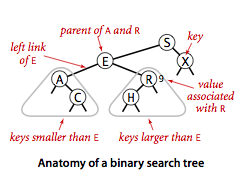
\includegraphics[scale=0.65]{img/bst-anatomy.png}
	\caption{BST anatomy.}
	\label{fig:bst-anatomy}
\end{figure}

\begin{myrem}
It's interesting to note that there are many different BSTs that
represent the same set.
\end{myrem}

\subsubsection{Basic implementation}
\begin{lstlisting}
public class BST<Key extends Comparable<Key>, Value>
{
	private Node root;
\end{lstlisting}

Just as we did for linked lists, we define a private nested class
to define nodes in BSTs.

\begin{lstlisting}
	public class Node {
		private Key key;
		private Value val;
		private Node left, right;
		private int N;
		
		public Node(Key key, Value val, int N) {
			this.key = key; this.val = val; this.N = N;		
		}	
	}
\end{lstlisting}

Each node contains a key, a value, a left and right link and a node
count. This last field facilitates the implementation of various
ordered symbol-table operations.

\begin{lstlisting}
	public int size() {
		return size(root);	
	}
	
	private int size(Node x) {
		if (x == null) return 0;
		else return x.N;	
	}
\end{lstlisting}

Thanks to the recursive definition of a tree, we can implement
the \lstinline{get()} easily in a recursive way.

\begin{lstlisting}
	public Value get(Key key) {
		return get(root, key);	
	}
	
	private Value get(Node x, Key key) {
		if (x == null) return null;
		
		int cmp = key.compareTo(x.key);
		if      (cmp > 0) return get(x.right, key);
		else if (cmp < 0) return get(x.left, key);
		else	 return x.val;
	}
\end{lstlisting} 

The same holds for the \lstinline{put()} method.

\begin{lstlisting}
	public void put(Key key, Value val) {
		root = put(root, key, val);	
	}
	
	private Node put(Node x, Key key, Value val) {
		if (x == null) return new Node(key, val, 1);
		
		int cmp = key.compareTo(x.key);
		if      (cmp > 0) x.right = put(x.right, key, val);
		else if (cmp < 0) x.left = put(x.left, key, val);
		else x.val = val;
		x.N = size(x.left) + size(x.right) + 1;
		return x;
	}
\end{lstlisting}

To get a better understanding of the dynamics of these
recursive implementations, you can think of the code
\textit{before} the recursive calls as happening on the
way \textit{down} the tree. Then, think of the code \textit{after}
the recursive calls as happeing on the way \textit{up} the tree.

Now, let's look at how to delete a node in a BST. This is the most
difficult operation to implement. We choose here to use the
\textit{Hibbard deletion}. With this method, we delete a node
$x$ by replacing it with its \textit{successor}. If $x$ has
a right child, its successor is the node with the smallest
key in its right subtree. This task is accomplished
in 4 steps :

\begin{itemize}
	\item Save a link to the node to be deleted in \lstinline{t} ;
	\item Set \lstinline{x} to point to its successor
	\lstinline{min(t.right)} ;
	\item Set the right link of \lstinline{x} to
	\lstinline{deleteMin(t.right)} ;
	\item Set the left link of \lstinline{x} to \lstinline{t.left}.
\end{itemize}

\begin{lstlisting}
	public void delete(Key key) {
		root = delete(root, key);	
	}
	
	private Node delete(Node x, Key key) {
		if (x == null) return null;
		int cmp = key.compareTo(x.key);
		if      (cmp < 0) x.left = delete(x.left, key);
		else if (cmp > 0) x.right = delete(x.right, key);
		else {
			if(x.right == null) return x.left;
			if(x.left == null) return x.right;
			/* Choose successor to replace x (Hibbard)
			if the node to delete has two children */
			Node t = x;
			x = min(t.right);
			x.right = deleteMin(t.right);
			x.left = t.left;		
		}	
		
		x.N = size(x.left) + size(x.right) +1;
		return x;
	}
\end{lstlisting}

Even though this method does the job, it has a flaw that might
cause performance problems in some practical situations. The problem
is that the choice of using the successor is arbitrary and not
symmetric. This will cause the BST to become skewed toward the
left on the long term for random deletions and insertions
\footnote{See the last video on 
\url{http://algs4.cs.princeton.edu/32bst/}.}.

\begin{myrem}
Note that deletion in a BST is not commutative. Try for
example to delete 4 and then 3 and 3 and then 4 in
the tree given in figure \ref{fig:nc-deletion}.

\begin{figure}[ht]
	\centering
	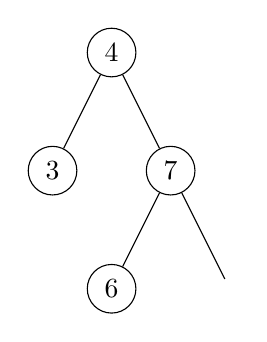
\begin{tikzpicture}
		\node [circle,draw] {4}
		child {node [circle,draw] {3}}
		child {node [circle, draw] {7}
			child {node [circle,draw] {6}}
			child {node [] {}}};
	\end{tikzpicture}
	\caption{Example of non-commutative deletion.}
	\label{fig:nc-deletion}
\end{figure}
\end{myrem}

\begin{myrem}
Others methods from the API are in the book.
\end{myrem}

\subsubsection{Analysis}
The running times of algorithms on binary search trees depend
on the shapes of the trees, which in turn, depend on the
order in which keys are inserted. In the best case, a tree
with $N$ nodes could be perfectly balanced, with $\log(n)$
nodes between the root and each null links (we call this the
\textit{depth} of a tree). In the worst case
there could be $N$ nodes on the search patch.

% Better to say "proposition" than "property" ? Do I need to change
% eplcommon.sty to add this?
\begin{myprop}
Search hits in BST build from $N$ random keys requires $\sim 2\log N$
(about $1.39\log(n)$) compares, on the average.
\end{myprop}

\begin{myprop}
Insertions and search misses in a BST build from $N$ random
keys require $\sim 2\log N$ (about $1.39\log(n)$) compares on the
average.
\end{myprop}

\begin{myprop}
In a BST, all operations take time proportional to the height of
the tree in the worst case.
\end{myprop}

\subsubsection{Binary tree traversal methods}
We will use the BST given in figure \ref{fig:bst-anatomy}
for the following examples and assume that the method
\lstinline$void visit(Node h)$ print the key of node
\lstinline$h$.

\paragraph{Preorder (\textit{préfixe)}}
Visit a node, then its left child and right child.
\begin{lstlisting}
public static void preOrder(Node h) {
	if(t != null) {
		visit(t);
		preOrder(t.left);
		preOrder(t.right);	
	}
}
\end{lstlisting}
Applied on figure \ref{fig:bst-anatomy} :
S E A C R H X.

\paragraph{Inorder (\textit{infixe})}
This method is equivalent to projecting the keys
of the tree on a line at the bottom of the tree :
\textbf{keys appear in sorted order}.

\begin{lstlisting}
public static void inOrder(Node h) {
	if(t != null) {
		inOrder(t.left);
		visit(t);
		inOrder(t.right);	
	}
}
\end{lstlisting}
Applied on figure \ref{fig:bst-anatomy} :
A C E H R S X.

\paragraph{Postorder (\textit{postfixe} ou \textit{suffice})}
Visit each node after having visited each children.
\begin{lstlisting}
public static void postOrder(Node h) {
	if(t != null) {
		postOrder(t.left);
		postOrder(t.right);
		visit(t);
	}
}
\end{lstlisting}
Applied on figure \ref{fig:bst-anatomy} :
C A R H E X S.

\subsection{Balanced search tree}
The algorithms in the previous subsection have poor worst-case,
performance. Here we introduce a type of binary search tree where
costs are \textit{guaranteed} to be logarithmic. Ideally, we would
like to keep our binary search tree perfectly balanced, i.e. in an
$N$-node tree, we would like the height to be $\log(N)$. Unfortunately,
maintaining this property is too expensive. Hence we will consider
a data structure that slightly relaxes the perfect balance
requirement to provide guaranteed logarithmic performance.

\begin{mydef}[2-3 search trees]
A \textit{2-3 search tree} is a tree that is either empty or
\begin{itemize}
	\item A \textit{2-node}, with one key (and associated value)
	and two links, a left link to 2-3 search tree with smaller
	keys, and a right link to a 2-3 search tree with larger keys ;
	\item A \textit{3-node}, with two keys (and associated values)
	and \textit{three} links, a left link to 2-3 search tree with
	smaller keys, a middle link to a 2-3 search tree with keys
	between the node's key, and a right link to a 2-3 search tree
	with larger keys.
\end{itemize}
As usual, we refer to a link to an empty tree as a \textit{null link}.
\end{mydef}

\begin{myprop}
A \textit{perfectly balanced} 2-3 search tree is one whose null
links are all the same distance from the root.
\end{myprop}

Searching in a 2-3 search tree is almost the same as searching
in a BST. The only difference occurs when we encounter a 3-node,
instead of just looking if the target key is smaller or lager
than the keys, we also have to check if the target key is
between the two keys of the 3-node.

Inserting in a 2-3 search tree is more complicated. The primary reason
that 2-3 trees are useful is that we can do insertions and still
maintain perfect balance. To achieve this, we have to take into
account different cases illustrated below 
(see figure \ref{fig:23tree-inserta}, \ref{fig:23tree-insertb}
and \ref{fig:23tree-insertc}).

\begin{myprop}
Transformations caused by the 2-3 tree insertion algorithms
are purely \textit{local}: no part of the tree needs to be examined
or modified other than the specified nodes and links. Moreover, these
local transformations preserve the global properties that the tree
is ordered and perfectly balanced.
\end{myprop}

\begin{myprop}
Search and insert operations in a 2-3 tree with $N$ keys are
guaranteed to visit at most $\log N$ nodes. Indeed, the height
of an $N$-node 2-3 tree is between $\log_3 N$ (if the tree is
all 3-nodes) and $\log N$ (if the tree is all 2-nodes).
\end{myprop}

\begin{figure}[ht]
	\centering
	\begin{subfigure}{.5\textwidth}
		\centering
  		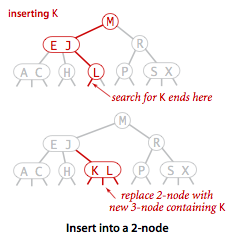
\includegraphics[width=.7\linewidth]{img/23tree-insert2.png}
 		\caption{Inserting into a 2-node.}
  		\label{fig:23tree-insert2}
	\end{subfigure}%
	\begin{subfigure}{.5\textwidth}
  		\centering
  		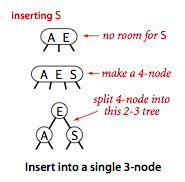
\includegraphics[width=0.5\linewidth]{img/23tree-insert3a.png}
  		\caption{Inserting into a single 3-node}
  		\label{fig:23tree-insert3a}
	\end{subfigure}
	\caption{}
	\label{fig:23tree-inserta}
\end{figure}

\begin{figure}[ht]
	\centering
	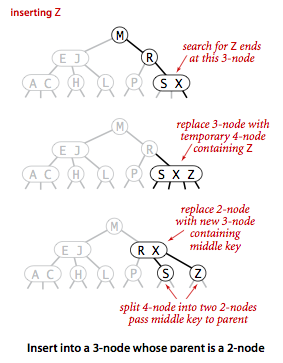
\includegraphics[scale=0.55]{img/23tree-insert3b.png}
	\caption{}
	\label{fig:23tree-insertb}
\end{figure}

\begin{figure}[ht]
	\centering
	\begin{subfigure}{.5\textwidth}
		\centering
  		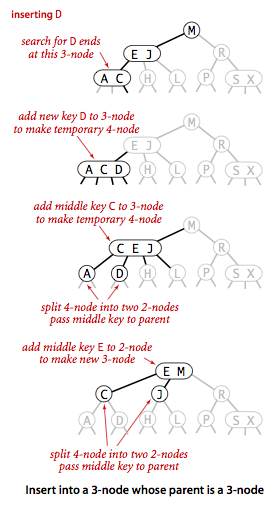
\includegraphics[width=.7\linewidth]{img/23tree-insert3c.png}
 		\caption{Insert intro a 3-node whose parent is a 3-node.}
  		\label{fig:23tree-insert3c}
	\end{subfigure}%
	\begin{subfigure}{.5\textwidth}
  		\centering
  		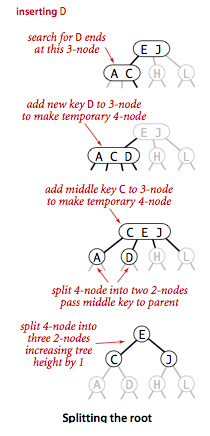
\includegraphics[width=0.6\linewidth]{img/23tree-split.png}
  		\caption{Splitting the root.}
  		\label{fig:23tree-split}
	\end{subfigure}
	\caption{}
	\label{fig:23tree-insertc}
\end{figure}

\subsubsection{Implementation}
To implement a 2-3 tree, we consider a simple representation
known as \textit{red-black BST}. The basic idea behind red-black
BSTs is to encode 2-3 tree by starting with standard BSTs and adding
extra information to encode 3-nodes. We think of the links as being of
two different type: \textit{red} links, which bind together two 2-nodes
to represent a 3-nodes, and \textit{black} links, which bind together
the 2-3 tree. Specifically, we represent 3-nodes as two 2-nodes connected
by a single red link that leans left. This is illustrated in figure
\ref{fig:redblack-encoding}.

One advantage of using such a representation is that it allows us
to use our \lstinline$get()$ code for standard BST search without
modification.

\begin{mydef}[Equivalent definition]
A red-black BST is a BST having red and black links and satisfying
the following three restrictions :
\begin{itemize}
	\item Red links lean left ;
	\item No node has two red links connected to it ;
	\item The tree has \textit{perfect black balance}: every path from
	the root to a null link has the same number of black links - we refer
	to this number as the tree's \textit{black height}.
\end{itemize}
\end{mydef}

\begin{myprop}
There is a 1-1 correspondence between red-black BSTs and 2-3 trees.
\end{myprop}

This last property is illustrated in figure \ref{fig:redblack-1-1}.

\begin{figure}[ht]
	\centering
	\begin{subfigure}{.5\textwidth}
		\centering
		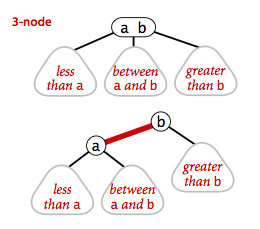
\includegraphics[scale=0.5]{img/redblack-encoding.png}
		\caption{Encoding a 3-node with two 2-nodes connected by
		a left leaning red link.}
		\label{fig:redblack-encoding}
	\end{subfigure}%
	\begin{subfigure}{.5\textwidth}
		\centering
		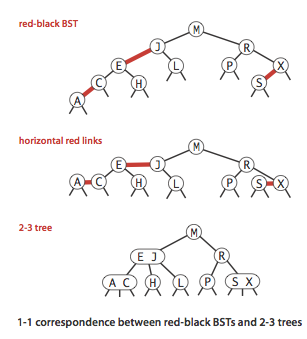
\includegraphics[scale=0.5]{img/redblack-1-1.png}
		\caption{1-1 correspondence between red-black BSTs and 2-3 trees.}
		\label{fig:redblack-1-1}
	\end{subfigure}
	\caption{}
	\label{fig:redblack-principles}
\end{figure}

\begin{lstlisting}
public class RedBlackBST<Key extends Comparable<Key>, Value>
{
	private Node root;
\end{lstlisting}

As usual, we define a private nested class to define a node.

\begin{lstlisting}
	private static final boolean RED = true;
	private static final boolean BLACK = false;
	
	private Class Node {
		Key key; Value val;
		Node left, right;
		int N;
		boolean color;	
	
		Node(Key key, Value val, int N, boolean color) {
			this.key = key; this.val = val;
			this.N = N; this.color = color;		
		}	
	}
	
	private boolean isRed(Node x) {
		if(x == null) return false;
		return x.color == RED;	
	}
\end{lstlisting}

When we refer to the color of a node, we are referring
to the color of the link pointing to it. By convention, null
links are black. Now we consider two methods
\lstinline$Node rotateLeft(Node h)$ and \lstinline$Node rotateRight(Node h)$.
These two methods will help us to write other methods later. They
are illustrated in figure \ref{fig:redblack-left-rotate} and
\ref{fig:redblack-right-rotate}.

\begin{figure}[ht]
	\centering
	\begin{subfigure}{.5\textwidth}
		\centering
		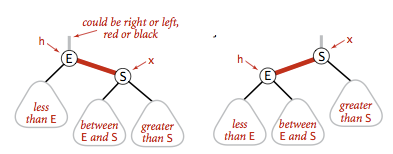
\includegraphics[scale=0.5]{img/redblack-left-rotate.png}
		\caption{Left rotate.}
		\label{fig:redblack-left-rotate}
	\end{subfigure}%
	\begin{subfigure}{.5\textwidth}
		\centering
		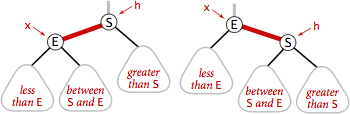
\includegraphics[scale=0.5]{img/redblack-right-rotate.png}
		\caption{Right rotate.}
		\label{fig:redblack-right-rotate}
	\end{subfigure}
	\caption{}
	\label{fig:redblack-rotations}
\end{figure}

\begin{lstlisting}
	private Node rotateLeft(Node h) {
		Node x = h.right;
		h.right = x.left; x.left = h;
		x.color = h.color; h.color = RED;
		x.N = h.N;
		h.N = 1 + size(h.left) + size(h.right);
		return x;
	}
	
	private Node rotateRight(Node h) {
		Node x = x.left;
		h.left = x.right; x.left = h;
		x.color = h.color; h.color = RED;
		x.N = h.N;
		h.N = 1 + size(h.left) + size(h.right);
		return x;
	}
\end{lstlisting}

Next we consider a simple method which allows us to
split a 4-node.

\begin{lstlisting}
	private void flipColors(Node h) {
		h.color = RED;
		h.left.color = BLACK;
		h.right.color = BLACK;	
	}
\end{lstlisting}

This method is illustrated in figure \ref{fig:color-flip}.

\begin{figure}[ht]
	\centering
	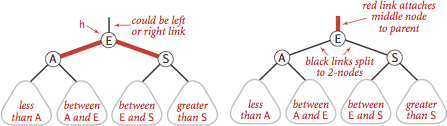
\includegraphics[scale=0.55]{img/color-flip.png}
	\caption{Flipping colors to split a 4-node.}
	\label{fig:color-flip}
\end{figure}

With the last three methods, we have everything we need to
implement insertion in red-black BSTs.

\begin{lstlisting}
	public void put(Key key, Value val) {
		root = put(root, key, val);
		root.color = BLACK;	
	}
	
	private Node put(Node h, Key key, Value val) {
		// Do standard insert, with red link to parent.
		if(h == null) return new Node(key, val, 1, RED);
		
		int cmp = key.compareTo(h.key);
		if      (cmp > 0) h.right = put(h.right, key, val);
		else if (cmp < 0) h.left = put(h.left, key, val);
		else h.val = val;
		
		if (isRed(h.left)  && isRed(h.left.left)) h = rotateRight(h);
		if (!isRed(h.left) && isRed(h.right))     h = rotateLeft(h);
		if (isRed(h.left)  && isRed(h.right))     flipColors(h);
		
		h.N = 1 + size(h.left) + size(h.right);
		return h:
	}	
\end{lstlisting}

A summary of rotations and colors flipping involved in insert is
given in figure \ref{fig:insert-summary}.

\begin{figure}[ht]
	\centering
	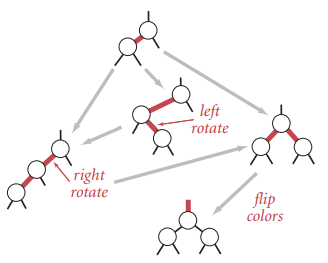
\includegraphics[scale=0.55]{img/insert-summary.png}
	\caption{Operations involved in insert.}
	\label{fig:insert-summary}
\end{figure}

% TODO : deletion in a red-bl	ack BST

\subsubsection{Analysis}
\begin{myprop}
The height\footnote{Here we are not talking about black height!} 
of a red-black BST with $N$ nodes
is no more than $2\log N$. Indeed, the worst case
is a 2-3 tree that is all 2-nodes except that the leftmost
is made up of 3-nodes. The path taking left links from the
root is twice as long as the path of length $\sim \log N$
that involves just 2-nodes.
\end{myprop}

The worst case of the last property corresponds to the first
tree of figure \ref{fig:redblack-1-1} with $S$ removed.

\begin{myprop}
The average length of a path from the root to a node
in a red-black BST with $N$ nodes is $\sim 1.00\log N$.
\end{myprop}

\begin{myprop}
In a red-black BST, the following operations take logarithmic time
in the worst case: search, insertion, finding the minimum/maximum,
floor, ceiling, rank, select, delete the minimum/maximum, delete
and range count.
\end{myprop}

\subsection{Hash tables}

If keys are small integers, we can use an array to implement
an unordered symbol table, by interpreting the key as an array
index so that we can store the value associated with the key
\lstinline$i$ in array entry \lstinline$i$, ready for
\textbf{immediate access}. Thanks to \textit{hashing}, we can
transform any type of key to array indexes. Ideally, different
keys would map to different indices. However, this ideal
is generally beyond our reach, so we have to face the possibility
that two or more different keys may hash to the same array index :
we need a \textit{collision resolution} process. We'll consider
two different approaches to collision resolution : \textit{separate
chaining} and \textit{linear probing}.

\subsubsection{Hash functions}

\begin{wrapfigure}{R}{0.3\textwidth}
  \begin{center}
    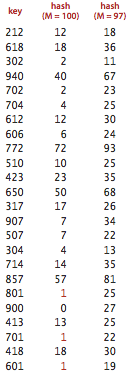
\includegraphics[width=0.15\textwidth]{img/modular-hashing.png}
  \end{center}
  \caption{Modular hashing.}
  \label{fig:modular-hashing}
\end{wrapfigure}

If we have an array that can hold $M$ key-value pairs, then we
need a hash function that can transform any given key into an
integer in the range $[0, M-1]$. We seek a hash function that both
is \textbf{efficient to compute} and \textbf{uniformly distributes}
the keys.

\paragraph{Hashing positive integers}
The most commonly used method for hashing integers is called
\textit{modular hashing}: we choose the array size $M$ to be prime
and, for any positive integer key $k$, compute the remainder
when dividing $k$ by $M$ : \lstinline$k % M$.

If $M$ is not prime, it may be the case that not all the bits
of the key play a role, which amounts to missing an opportunity
to disperse the values evenly. For example, if the keys are
base 10 numbers and $M$ is $10^k$, then only the $k$ least
significant digits are used (see figure \ref{fig:modular-hashing}).

\paragraph{Hashing floating-point numbers}
One way to do this is to use modular hashing on the binary
representation of the key (this is what Java does).

\paragraph{Hashing strings}
Again, we can apply modular hashing on each character of
the string :

\begin{lstlisting}
int hash = 0;
for(int i = 0; i < s.length(); i++)
	hash = (R * hash + s.charAt(i)) % M;
\end{lstlisting}

This algorithm is called the \textit{Horner's method}.
The use of a small primer integer such as 31 ensures
that the bits of all the characters play a role.

\begin{myrem}
\label{rem:mod-prop}
Note that applying \lstinline|% M| at the end (i.e. outside
the loop) gives the same result (it's a property of the
modulus operation). But by doing so, we may encounter
\lstinline|int| overflow for long strings.
\end{myrem}

\paragraph{Java conventions}
In Java, every data type inherits a method called
\lstinline$hashCode()$ that returns a 32-bit integer.
The implementation of \lstinline$hashCode()$ for a data
type must be \textbf{consistent with equals}, if
\lstinline$a.equals(b)$, then \lstinline$a.hashCode()$
must have the same numerical value as
\lstinline$b.hashCode()$. Conversely, if
\lstinline$hashCode()$ values
are different, then objects are different. \textbf{But},
if \lstinline$hashCode()$ values are the same, we still
have to use \lstinline$equals()$ to check whether or not
objects are equal (as collisions may occur).

\paragraph{Converting a hashcode to an array index}
Since our goal is an array index, not a 32-bit integer, we
combine \lstinline$hashCode()$ with modular hashing
to produce integers between 0 and $M-1$ :

\begin{lstlisting}
private int hash(Key x) {
	return (x.hashCode() && 0x04fffffff) % M);
}
\end{lstlisting}

This code also masks off the sign bit (to turn the
32-bit number into a 31-bit non-negative integer).
We usually use a prime number for the hash table
size $M$ to attempt to make use of all the bits of
the hash code.

\paragraph{Software caching}
If computing the hash code is expensive, it may be
worthwhile to \textit{cache the hash} for each key.
That is, we maintain an instance variable \lstinline$hash$
in the key type that contains the value of
\lstinline$hashCode()$ for each key object. Java uses
this technique for \lstinline$String$ objects.

\subsubsection{Hashing with separate chaining}
Now that we know how to hash, we need a collision resolution
process. The first collision resolution process is illustrated
in figure \ref{fig:separate-chaining}.

\begin{figure}[ht]
	\centering
	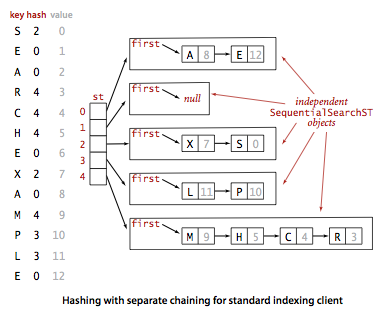
\includegraphics[scale=0.6]{img/separate-chaining.png}
	\caption{For each of the $M$ array indices, we build a 
	linked list of the key-value pairs  whose key hash to that
	index. To search in those linked lists, we use sequential
	search in an unordered linked list.}
	\label{fig:separate-chaining}
\end{figure}

\paragraph{Implementation}
Implementation of separate chaining is very easy
(\lstinline|SequentialSearchST| is the implementation
of the sequential search in an unordered linked list).

\begin{lstlisting}
public class SeparateChainingHashST<Key, Value> 
{
	private int M;
	private SequentielSearchST<Key, Value>[] st;
	
	public SeparateChainingHashST() {
		this(997);	
	}
	
	public SeparateChainingHashST(int M) {
		this.M = M;
		st = (SequentielSearchST<Key, Value>[]) new SequentialSearchST[M];
		for(int i = 0; i < M; i++) {
			st[i] = new SequentialSearchST();		
		}	
	}
	
	private int hash(Key key) {
		return (key.hashCode() & 0x7fffffff) % M;	
	}
	
	public Value get(Key key) {
		return (Value) st.[hash(key)].get(key);	
	}
	
	public void put(Key key, Value val) {
		st[hash(key)].put(key, val);	
	}
}
\end{lstlisting}

\paragraph{Analysis}
\begin{myprop}
In a separate-chaining hash table with $M$ lists and $N$
keys, the probability that the number of keys in a list
is within a small constant factor of $N/M$ is extremely
close ton 1.
\end{myprop}

This last property makes the assumption that we use
a uniform hashing function.

\begin{myprop}
As a consequence of the last property, the number of
compares for search miss and insert is $\sim N/M$.
\end{myprop}

\subsubsection{Hashing with linear probing}
Another approach to implementing hashing is to store
$N$ key-value pairs in a hash table of size $M > N$,
relying on empty entries in the table to help with
collision resolution. Such methods are called
\textit{open-addressing} hashing methods. The simplest
one is called linear probing : when there is a collision,
then we just check the next entry in the table.

\paragraph{Implementation}
As with separate chaining, implementation is quite
straightforward.

\begin{lstlisting}
public class LinearProbingHashST<Key, Value>
{
	private int N; // number of key-value pairs in the table
	private int M; // size of linear-probing table
	private Key[] keys;
	private Values[] vals;
	
	public LinearProbingHashST() {
		this(4); // Initializes with an initial capacity of 4	
	}	
	
	public LinearProbingHashST(int capacity) {
		M = capacity;		
		keys = (Key[]) new Object[M];
		vals = (Value[]) new Object[M];	
	}
	
	private int hash(Key key) {
		return (key.hashCode() &0x7fffffff) % M;	
	}
	
	public void put(Key key, Value val) {
		if(N >= M/2) resize(2*M);
		
		int i;
		for(i = hash(key); keys[i] != null; i = (i + 1) % M) {
			if(keys[i].equals(key)) {
				vals[i] = val;
				return;
			}		
		}	
		
		keys[i] = key;
		vals[i] = val;
		N++;
	}
	
	public Value get(Key key) {
		for(int i = hash(key); keys[i] != null; i = (i + 1) % M) {
			if(keys[i].equals(key)) {
				return vals[i];			
			}
		}
		
		return null;	
	}
	
	public void delete(Key key) {
		if(!contains(key)) return;
		int i = hash(key);
		while(!key.equals(keys[i]))
			i = (i + 1) % M;
		keys[i] = null;
		vals[i] = null;
		i = (i + 1) % M;
		while(keys[i] != null) {
			Key keyToRedo = keys[i];
			Value valtoRedo = vals[i];
			keys[i] = null;
			vals[i] = null;
			N--;
			put(keyToRedo, valToRedo);
			i = (i + 1) % M;		
		}
		
		N--;
		if(N > 0 && M <= M/8)
			resize(M/2);
	}
\end{lstlisting}

\begin{mydef}
We define $\alpha = N/M$ as the \textit{load factor}
of a hash table. For separate chaining, $\alpha$ is
the average number of keys per list and is often
larger than 1. For linear probing, $\alpha$ is the
percentage of table entries that are occupied : it
cannot be greater than 1\footnote{If the load
factor reach 1, search miss would go into an
infinite loop.}.
\end{mydef}

The average cost of linear probing depends on \textit{clusters}
(entries which clump together into contiguous groups).
For the sake of good performance, we use array resizing
to guarantee that the load factor is between $\frac{1}{8}$
and $\frac{1}{2}$ : this allows us to avoid too long clusters.
The \lstinline|resize| method is given below.

\begin{lstlisting}
	private void resize(int cap) {
		LinearProbingHashST<Key, Value> t;
		t = new LinearProbingHashST<Key, Value>(cap);
		for(int i = 0; i < M; i++) {
			if(keys[i] != null) {
				t.put(keys[i], vals[i]);			
			}		
		}
		
		keys = t.keys;
		vals = t.vals;
		M = t.M;	
	}
}
\end{lstlisting}


\subsection{Summary}
The cost-summary for symbol-tables implementations is given
in table \ref{tab:cost-summary-searching}.

% auto-generated from here http://www.tablesgenerator.com/ #flemme
\begin{table}[ht]
\centering
\begin{tabular}{c|ccccc}
\multirow{2}{*}{\begin{tabular}[c]{@{}c@{}}algorithm \\(data structure)\end{tabular}} &
\multicolumn{2}{c}{\begin{tabular}[c]{@{}c@{}}worst-case cost\\ (after N inserts)\end{tabular}} &
\multicolumn{2}{c}{\begin{tabular}[c]{@{}c@{}}average-case cost\\ (after N random inserts)\end{tabular}} &
\multirow{2}{*}{\begin{tabular}[c]{@{}c@{}}efficiently support\\ordered operations?\end{tabular}} \\
& search & insert & search hit & insert &  \\ \hline
\begin{tabular}[c]{@{}c@{}}sequential search\\
(unordered linked list)\end{tabular} & $N$ & $N$ & $N/2$ & $N$ & no  \\
\begin{tabular}[c]{@{}c@{}}binary search\\ 
(ordered array)\end{tabular} & $\log N$ & $N$ & $\log N$ & $N/2$ & yes \\
\begin{tabular}[c]{@{}c@{}}binary tree search\\ 
(BST)\end{tabular} & $N$ & $N$ & $1.39 \log N$ & $1.39 \log N$ & yes \\
\begin{tabular}[c]{@{}c@{}}2-3 tree search\\
(red-black BST)\end{tabular} & $2 \log N$ & $2 \log N$ & $1.00 \log N$ & $1.00 \log N$ & yes \\                                                                                                 
\begin{tabular}[c]{@{}c@{}}separate chaining\\
(array of lists)\end{tabular} & $N$ & $N$ & $\frac{N}{2M}$ & $N/M$ & no \\
\begin{tabular}[c]{@{}c@{}}linear probing\\
(parallel arrays)\end{tabular} & $N$ & $N$ & $< 1.50$ & $< 2.50$ & no                                                                                                 
\end{tabular}
\caption{Cost summary for symbol-table implementations.}
\label{tab:cost-summary-searching}
\end{table}

\section{Strings}
\subsection{Tries}
\paragraph{Goals}
As with sorting, we can take advantage of properties of strings to develop search meth-
ods (symbol-table implementations) that can be more efficient for typical applications where search keys are strings.
More specifically, the goals are the next-ones: 
\begin{itemize}
\item{Search hits take time proportional to the length of the search key.}
\item{Search misses involve examining only a few characters.}
\end{itemize}

To achieve it, we have to adjust the symbol-table API (cfr fig \ref{triesAPI}) to provide specific character-based operations for string keys.

\begin{figure}[ht!]
\centering
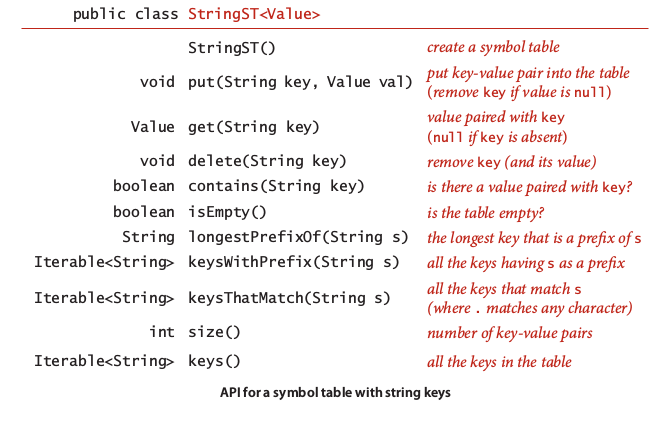
\includegraphics[width=.7\linewidth]{img/APItries.png}
\caption{Tries API}
\label{triesAPI}
\end{figure}

Considering the following example keys: she sells sea
shells by the sea shore ,let's focus on the addition of three new method: \begin{itemize}
\item{\textbf{{\textit{longuestPrefixOf()}}}: takes a string as argument and returns the longest
key in the symbol table that is a prefix of that string. For the given keys,
longestPrefixOf("shell") is she and longestPrefixOf("shellsort") is
shells .}
\item{\textbf{{\textit{keysWithPrefix()}}} takes a string as argument and returns all the keys
in the symbol table having that string as prefix. For the given keys,
keysWithPrefix("she") is she and shells , and keysWithPrefix("se") is
sells and sea .}
\item{\textbf{{\textit{keysThatMatch()}}} takes a string as argument and returns all the keys in the
symbol table that match that string, in the sense that a period (.) in the argu-
ment string matches any character. For the given keys, keysThatMatch(".he")
returns she and the , and keysThatMatch("s..") returns she and sea .}
\end{itemize}

\subsubsection{Basic Tries}

\begin{mydef}[Tries]
A \textit{trie} is a search tree build from the characters of the string keys that allows the use the characters of the search
key to guide the search. A trie has the same structure as a search tree. We usually omit null links due to a substantial number of these one. Each node corresponds to a character value (except the root) and is associated to a value, which can be \textit{null} or the value associated to one of the string key of the symbol table. A representation is given fig \ref{Basic trie}.
\end{mydef}


\begin{figure}[ht!]
\centering
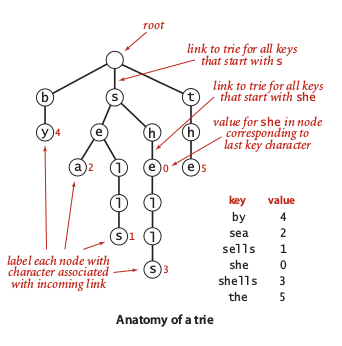
\includegraphics[width=.4\linewidth]{img/tries.png}
\caption{Basic trie}
\label{Basic trie}
\end{figure}

\paragraph{Search}
Due to this organisation, search in tree is very easy: beginning at the root, following the path made by the characters inside the nodes until reaching the last character of the key is the only thing you have to do. Null links may be found if the next desired character isn't in the trie. Three results can occur:
\begin{itemize}
\item{The value at the node corresponding to the last character in the key is not null: this result is
a \textbf{search hit}. The value associated with the key is the value in the node corre-
sponding to its last character.}
\item{The value in the node corresponding to the last character in the key is null (as
in the search for shell depicted at top right above). This result is a \textbf{search miss}:
the key is not in the table.}
\item{The search terminated with a null link (as in the search for shore depicted at
bottom right above). This result is also a \textbf{search miss}.}
\end{itemize}

An example of search is given fig \ref{Search in a basic trie}.

\begin{figure}[ht!]
\centering
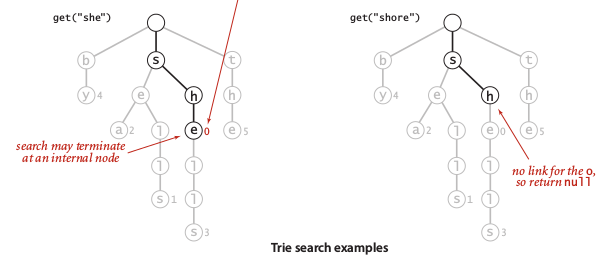
\includegraphics[width=.75\linewidth]{img/trieSe.png}
\caption{Search in a basic trie}
\label{Search in a basic trie}
\end{figure}

\paragraph{Insertion}
To insert a value, we begin by doing a search: we go down the trie, guided by the character of the key. Two situations can occur:
\begin{itemize}
\item{\textbf{Null link encountered}: a null link is encountered before reaching the last character of the key. This implies that there is no node corresponding to this one and we have thus to create a new node for each remaining character of the key. The value is set in the node of the last character.}
\item{\textbf{Last character encountered}: the last character of the key is encountered before reaching a null link. We just have to set the node's value to the value corresponding to the key.}
\end{itemize}

An example of insertion in a basic trie is given fig \ref{Insertion in a basic trie}.

\begin{figure}[ht!]
\centering
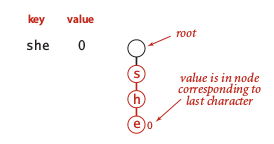
\includegraphics[width=.4\linewidth]{img/trieIn1.png}
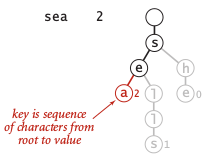
\includegraphics[width=.3\linewidth]{img/trieIn2.png}
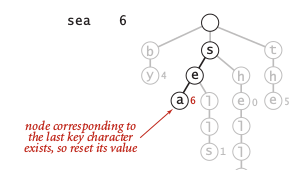
\includegraphics[width=.4\linewidth]{img/trieIn3.png}
\caption{Insertion in a basic trie}
\label{Insertion in a basic trie}
\end{figure}

\paragraph{Implementation}
A implementation of a trie is given below:
\begin{lstlisting}
public class TrieST<Value>
{

private static int R = 256; // radix
private Node root;
// root of trie

private static class Node
{
	private Object val;
	private Node[] next = new Node[R];
}

public Value get(String key)
{
	Node x = get(root, key, 0);
	if (x == null) return null;
	return (Value) x.val;
}

private Node get(Node x, String key, int d)
{ // Return value associated with key in the subtrie rooted at x.
	if (x == null) return null;
	if (d == key.length()) return x;
	char c = key.charAt(d); // Use dth key char to identify subtrie.
	return get(x.next[c], key, d+1);
}

public void put(String key, Value val)
{ root = put(root, key, val, 0); }

private Node put(Node x, String key, Value val, int d)
{ // Change value associated with key if in subtrie rooted at x.
	if (x == null) x = new Node();
	if (d == key.length()) { x.val = val; return x; }
	char c = key.charAt(d); // Use dth key char to identify subtrie.
	x.next[c] = put(x.next[c], key, val, d+1);
	return x;
}
}
\end{lstlisting}

\paragraph{Collecting keys}
Because keys are represented implicitly in the trie, it is difficult to provide to user the ability to iterate through the keys. We do not use a queue to stock the different keys as with the binary search tree but we create a explicit representation of all the string keys using the recursive method \textit{collect()}. This method visits the differents nodes and appends the corresponding characters to create the keys. The \textit{collect()} method is use to implements the \textit{keysWithPrefix()} method which is used to implements the \textit{keys()} method. The last one allow to create all the different keys (exemple given fig \ref{keysRe}). A implementation of the  \textit{collect()}, \textit{keysWithPrefix} and \textit{keys()} methods are given below: 

\begin{lstlisting}
public Iterable<String> keys()
{ return keysWithPrefix(""); }

public Iterable<String> keysWithPrefix(String pre)
{
	Queue<String> q = new Queue<String>();
	collect(get(root, pre, 0), pre, q);
	return q;
}

private void collect(Node x, String pre, Queue<String> q)
{
	if (x == null) return;
	if (x.val != null) q.enqueue(pre);
	for (char c = 0; c < R; c++)
		collect(x.next[c], pre + c, q);
}
\end{lstlisting} 

The \textit{keysThatMatch()} method use the similar process, but add an argument to specify the pattern to collect. A possible implementation is given below:

\begin{lstlisting}
public Iterable<String> keysThatMatch(String pat)
{
	Queue<String> q = new Queue<String>();
	collect(root, "", pat, q);
	return q;
}

public void collect(Node x, String pre, String pat, Queue<String> q)
{
	int d = pre.length();
	if (x == null) return;
	if (d == pat.length() && x.val != null) q.enqueue(pre);
	if (d == pat.length()) return;
	char next = pat.charAt(d);
	for (char c = 0; c < R; c++)
		if (next == '.' || next == c)
			collect(x.next[c], pre + c, pat, q);
}
\end{lstlisting}

The \textit{longuestPrefix()} method first looks for the biggest length found for a path that matches with the parameter string and then return a substring with the obtained length

\begin{lstlisting}
public String longestPrefixOf(String s)
{
	int length = search(root, s, 0, 0);
	return s.substring(0, length);
}

private int search(Node x, String s, int d, int length)
{
	if (x == null) return length;
	if (x.val != null) length = d;
	if (d == s.length()) return length;
	char c = s.charAt(d);
	return search(x.next[c], s, d+1, length);
}
\end{lstlisting}

\begin{figure}[ht!]
\centering
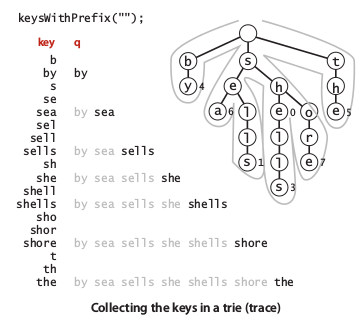
\includegraphics[width=.45\linewidth]{img/keysRe.png}
\caption{Keys recuperation}
\label{keysRe}
\end{figure}

\paragraph{Deletion}
AS for the insertion, the first step of a deletion is a search: the goal is to find the node corresponding to the key and set its value to null. Two situations may occur then:
\begin{itemize}
\item{The node has non-null link to a child. No more work is required}
\item{All the remaining link are null. We have thus to remove the node. Caution that if doing so leaves all the links null in its parent, we need to remove that node,
and so forth.}
\end{itemize}
A exemple is given fig \ref{trieDel}. A possible implementation is given below:
\begin{lstlisting}
public void delete(String key)
{ root = delete(root, key, 0); }

private Node delete(Node x, String key, int d)
{
	if (x == null) return null;
	if (d == key.length())
		x.val = null;
	else
	{
		char c = key.charAt(d);
		x.next[c] = delete(x.next[c], key, d+1);
	}
	
	if (x.val != null) return x;
	
	for (char c = 0; c < R; c++)
		if (x.next[c] != null) return x;
	return null;
}
\end{lstlisting}

\begin{figure}[ht!]
\centering
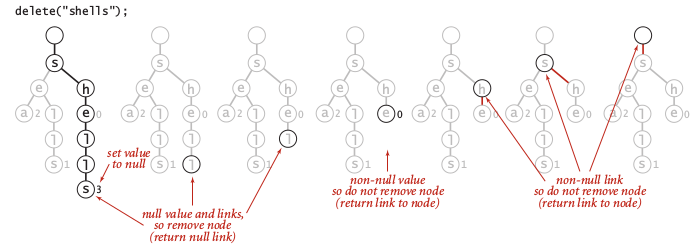
\includegraphics[width=.75\linewidth]{img/trieDel.png}
\caption{Deletion with basic trie}
\label{trieDel}
\end{figure}

\begin{myprop}
The linked structure (shape) of a trie is independent of the key in-
sertion/deletion order: there is a unique trie for any given set of keys.
\end{myprop}

\begin{myprop}
The number of array accesses when searching in a trie or inserting
a key into a trie is at most 1 plus the length of the key. From a theorical point of view, this implies that tries are optimal for search hit.
\end{myprop}

\begin{myprop}
The average number of nodes examined for search miss in a trie
built from N random keys over an alphabet of size R is ~log R N .
\end{myprop}

\begin{myprop}
The number of links in a trie is between RN and RNw, where w is
the average key length. More precisely, for $N$ random keys and $w$ the average length of a key, we can proove that:
\begin{itemize}
\item{When keys are short, the number of links is close to RN.}
\item{When keys are long, the number of links
is close to RNw.}
\item{Therefore, decreasing R can save a huge
amount of space.}
\end{itemize}
\end{myprop}

\paragraph{Size}
On average, the required space for a trie is huge due to the one-way-branching that can occur. A solution to this problem is the \textit{ternary search trie}.

\subsubsection{Ternary search tries (TST)}

\begin{mydef}
A \textit{ternary search trie} is a trie in which each node has a character, three links,
and a value. The three links correspond to keys
whose current characters are less than, equal
to, or greater than the node’s character. In TST, characters appear explicitly in nodes: we
find characters corresponding to keys only
when we are traversing the middle links.
\end{mydef}

\paragraph{Search}
Due to this configuration, a search appears to be easy: we compare the
first character in the key with the character at
the root. If it is less, we take the left link; if it is
greater, we take the right link; and if it is equal,
we take the middle link and move to the next
search key character. The algorithm is applied recursively.

\paragraph{Insertion}
The insertion is like an insertion for tries: beginning with a search and then add the value in a new node or not. A example is given fig \ref{TSTSe}.

\begin{figure}[ht!]
\centering
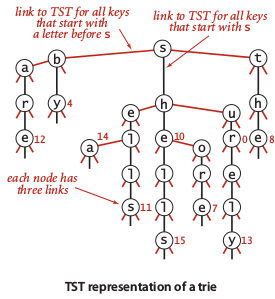
\includegraphics[width=.4\linewidth]{img/TST.png}
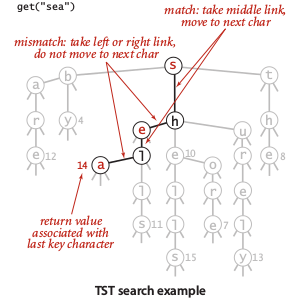
\includegraphics[width=.4\linewidth]{img/TSTSe.png}
\caption{TST representation and search}
\label{TSTSe}
\end{figure}

Using this arrangement is equivalent to implementing
each R-way trie node as a binary search tree that uses
as keys the characters corresponding to non-null links.
Continuing the correspondence, TSTs correspond to 3-way string quicksort (cfr fig \ref{TSTnode}).

\begin{figure}[ht!]
\centering
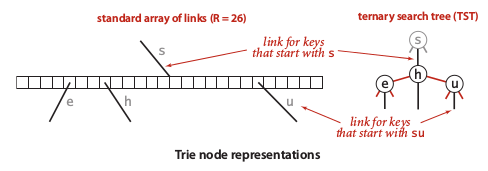
\includegraphics[width=.75\linewidth]{img/TSTnode.png}
\caption{Node representation of a TST}
\label{TSTnode}
\end{figure}

\paragraph{Immplementation}
A implementation is given below:

\begin{lstlisting}
public class TST<Value>
{

private Node root;
private class Node
{
	char c;
	Node left, mid, right;
	Value val;
}

public Value get(String key)
// root of trie
// character
// left, middle, and right subtries
// value associated with string
// same as for tries (See page 737).
private Node get(Node x, String key, int
{
	if (x == null) return null;
	char c = key.charAt(d);
	if(c < x.c) return get(x.left, key, d);
	else if (c > x.c) return get(x.right, key, d);
	else if (d < key.length() - 1)
		return get(x.mid, key, d+1);
	else return x;
}

public void put(String key, Value val)
{ root = put(root, key, val, 0); }

private Node put(Node x, String key, Value val, int d)
{
	char c = key.charAt(d);
	if (x == null) { x = new Node(); x.c = c; }
	if(c < x.c) x.left = put(x.left, key, val, d);
	else if (c > x.c) x.right = put(x.right, key, val, d);
	else if (d < key.length() - 1)
	x.mid= put(x.mid,key, val, d+1);
	else x.val = val;
	return x;
}
}
\end{lstlisting}

\begin{myprop}
The number of links in a TST built from N string keys of average
length w is between 3N and 3Nw. This implies that the required space for a TST is well-over shorter than for a basic trie.
\end{myprop}

\begin{myprop}
A search miss in a TST built from N random string keys requires on the average $\sim ln N$ character compares:  search hit or an insertion in a TST uses
a character compare for each character in the search key.
\end{myprop}

In the worst case, a node might be a full R-way node that is unbalanced, stretched out
like a singly linked list, so we would need to multiply by a factor of R.

\paragraph{Alphabets}
The prime virtue of using TSTs is that they adapt gracefully to irregularities
in search keys. First, we usually use large alphabets  in pratictal applications. These alphabet may be a problem when using a basic tree due to a huge amount of link. With TST, we can use a 256-character ASCII encoding or a 65,536-character
Unicode encoding without having to worry about the excessive costs of nodes with 256-
or 65,536-way branching, and without having to determine which sets of characters are
relevant. 

\paragraph{Prefix match, collecting keys, and wildcard match.}
A TST represent a trie, so \textit{longuestPrefixOf()}, \textit{keys()}, \textit{keysWithPrefix()} ans \textit{keysThatMatch()} implementation can be easily adapted.

\paragraph{Deletion}
Deletion for a TST require more work: du to his organisation, we have to use the BST node deletion method.

\paragraph{Improvement: Hybrid TSTs}
An easy improvement can be made by using large explicit multiway node at the root (by keeping a table of $R$ TST by example). For this method to be effective, the leading digits of the keys must be well distributed.The resulting hybrid tries 
algorithm corresponds to the way that a human might search for names in a telephone
book ("Beginning by 'A', before 'Andrews' but after 'Aindan'").

\paragraph{One-way-branching} Just as with tries, we can make TSTs more efficient in their use of
space by putting keys in leaves at the point where they are distinguished and by eliminating one-way branching between internal nodes. we have thus the next proposition:
a search or an insertion in a TST built from N random string keys
with no external one-way branching and $R^t$ -way branching at the root requires
roughly ln N - t ln R character compares, on the average.

\paragraph{Performance point of view}
If space is available, R-way tries provide the fastest search, essentially completing the
job with a constant number of character compares. For large alphabets, where space
may not be available for R-way tries, TSTs are preferable, since they use a logarithmic
number of character compares, while BSTs use a logarithmic number of key compares.

\begin{figure}[ht!]
\centering
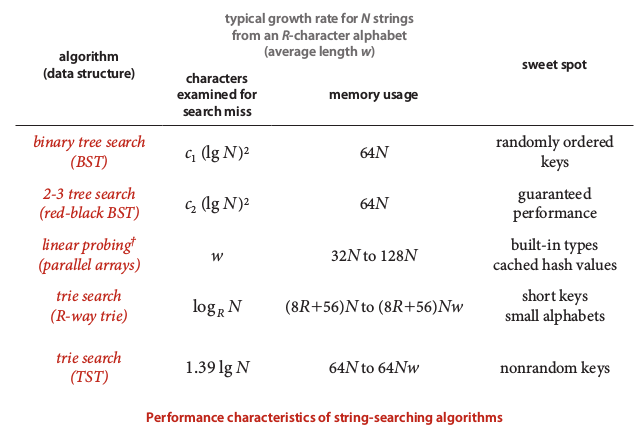
\includegraphics[width=.75\linewidth]{img/perf.png}
\label{perf}
\end{figure}

\subsection{Substring search}
\begin{myprob}[Substring search]
Given a \textit{text} string of length $N$ and
a pattern string of length $M$, find an occurence
of the pattern within the text.
\end{myprob}

\subsubsection{Rabin-Karp finger print search}
The Rabin-Karp algorithm uses hashing to solve this problem.
It's almost as simple as the brute-force algorithm but
runs in time proportional to $M+N$ with very high probability.
Furthermore, this algorithm extends to two-dimensional patterns,
which makes it more useful than the others for image processing.

\paragraph{Basic idea}
The basic idea behind this algorithm is the following : we compute
a hash function for the pattern an then look for a match by using
the same hash function for each possible $M$ character substring
of the text. If we find a text substring with the same hash value
as the pattern, we can check for a match. 

\paragraph{Key idea}
A straightforward implementation based on this description would be much
slower than a brute-force search (since computing a hash function that involves
every character is likely to be much more expensive than just
comparing characters). But Rabin and Karp showed that it is easy
to compute hash functions for $M$-characters substrings in
constant time, which leads to a linear-time substring search.

Using the notation $t_i$ for \lstinline|txt.charAt(i)|, the number
corresponding to the $M$-character substring of \lstinline|txt| that
starts at position \lstinline|i| using Horner's method is

\[ x_i = t_iR^{M-1} + t_{i+1}R^{M-2} + \dots + t_{i+M-1}R^0 \]

and we can assume that we know the value of $h(x_i) = x_i\mod Q$.
Shifting one position right in the text corresponds to replacing
$x_i$ by

\[ x_{i+1} = (x_i - t_iR^{M-1})R + t_{i+M}. \]

We substract off the leading digit, multiply it by $R$, then add
the trailing digit. Now, the crucial point is that we do not have
to maintain the values of the numbers (i.e. $x_i$), just the
values of theirs reminders when divided by $Q$ (i.e. $h(x_i)$).
Remember the property of modulus operation discussed in remark
\ref{rem:mod-prop}.

\paragraph{Implementation}
Here is the implementation of the \textit{Monter Carlo}
version of the Rabin-Karp fingerprint substring search.

\begin{mydef}
A \textit{Monte Carlo} algorithm is a randomized algorithm
whose running time is deterministic, but whose output may be
incorrect with a certain probability. On the other side, a
\textit{Las Vegas} algorithm is a randomized algorithm that
always gives correct results.
\end{mydef}

\begin{lstlisting}
public class RabinKarp
{
	private long patHash; // pattern hash value
	private int M; // pattern length
	private long Q; // a large prime
	private int R = 256; // alphabet size
	private long RM; // R^(M-1) % Q for use in removing leading digit
	
	public RabinKarp(String pat) {
		M = pat.length();
		Q = longRandomPrime();
		RM = 1;
		for (int i = 1; i <= M-1; i++) {
			RM = (R * RM) % Q;		
		}
		
		patHash = hash(pat, M);
	}
	
	private long hash(String key, int M) {
		long h = 0;
		for(int j = 0; j < M; j++) {
			h = (R * h + key.charAt(j)) % Q;		
		}
		
		return h;
	}
	
	private int search(String txt) {
		int N = txt.length();
		long txtHash = hash(txt, M);
		
		if(patHash == txtHash)	return 0; // match
		
		for(int i = M; i < N; i++) {
			txtHash = (textHash + Q - RM*txt.charAt(i-M) % Q) % Q;
			txtHash = (textHash*R + txt.charAt(i)) % Q;
			if(patHash == txtHash)
				return (i - M + 1);		
		}
		
		return N; // no match
	}
}
\end{lstlisting}

\begin{myrem}
An extra \lstinline|Q| is added on line 36 to make sure that
everything is positive so that the remainder operation works as
it should.
\end{myrem}

By choosing a value of \lstinline|Q| greater than $10^{20}$, we
reduce the risk of collision, and thus reduce the probability
of the Monte Carlo algorithm to fail. The alternative method
of checking for a match could be slow but is guaranteed correct.

\subsection{Data compression}
\begin{myprob}[Lossless compression]
The objectives of data compression is to obtain two black boxes :
\begin{itemize}
	\item A \textit{compress} box that transforms a bitstream $B$
	into a compressed version $C(B)$ ;
	\item An \textit{expand} box that transforms $C(B)$ back into $B$.
\end{itemize}
Using the notation $|B|$ to denote the number of bits in bitstream,
we are interested in minimizing the quantity $|C(B)|/|B|$, which is
known as the compression ratio.
\end{myprob}

\begin{myprop}
Universal data compression is impossible, that is, no algorithm
can compress every bitstream.
\end{myprop}

\subsubsection{Huffman compression}
The idea is to abandon the way in which text files are
usually stored: instead of using the usual 7 or 8 bits
for each character, we use fewer bits for characters that
appear often than for those that appear rarely.

A \textit{code} associates each character with a bitstring:
a symbol table with characters as keys and bitstrings as values.

Then, we take advantage of the fact that \textit{delimiters
are not needed if no character code is is the prefix of
another}. A code with this property is known as \textit{prefix
-free code}. All prefix-free codes are \textit{uniquely decodable}
(without needing any delimiters).

One convenient way to represent a prefix-free code is with
a trie. The general method for finding the optimal prefix-free
code is the hearth of Huffman compression.

\paragraph{Overview}
To compress a bitstream :
\begin{itemize}
	\item Read the input ;
	\item Tabulate the frequency of occurrence of each
	char value in the input ;
	\item Build the Huffman encoding trie corresponding to
	those frequencies ;
	\item Build the corresponding codeword table to associate
	a bitstring with each \lstinline|char| value in the input ;
	\item Write the trie, encoded as bitstring ;
	\item Write the count of characters in the input, encoded
	as a bitstring ;
	\item Use the codeword table to write the codeword for each
	input character.
\end{itemize}

To expand a bitstream :
\begin{itemize}
	\item Read the trie (encoded at the beginning of the bistream ;
	\item Read the count of characters to be decoded ;
	\item Use the trie to decode the bitstream.
\end{itemize}

\section{Graphs}

\subsection{Graphe non-orienté}

\paragraph{Definition}
A graph is a set of vertices and a collection of edges that each connect a
pair of vertices.

\paragraph{Anomalies}
Our definition allows two simple anomalies:
\begin{itemize}

\item A self-loop is an edge that connects a vertex to itself.
\item Two edges that connect the same pair of vertices are parallel.

\end{itemize}



\paragraph{Definition}

A path in a graph is a sequence of vertices
connected by edges. A simple path is one with no repeated
vertices. A cycle is a path with at least one edge whose first
and last vertices are the same. A simple cycle is a cycle with
no repeated edges or vertices (except the requisite repetition
of the first and last vertices). The length of a path or
a cycle is its number of edges.

\paragraph{Definition}

A graph is connected if there is a path from every vertex to every other
vertex in the graph. A graph that is not connected consists of a set of connected components,
which are maximal connected subgraphs.

\paragraph{Definition}

A tree is an acyclic connected graph. A disjoint
set of trees is called a forest. A spanning tree of a
connected graph is a subgraph that contains all of that
graph’s vertices and is a single tree. A spanning forest of
a graph is the union of spanning trees of its connected
components.

For example, a graph G with V vertices is a tree if and
only if it satisfies any of the following five conditions:

\begin{itemize}
\item G has V-1 edges and no cycles.
\item G has V-1 edges and is connected.
\item G is connected, but removing any edge disconnects it.
\item G is acyclic, but adding any edge creates a cycle.
\item Exactly one simple path connects each pair of vertices in G.
\end{itemize}

\paragraph{Definition}

A bipartite graph is a graph whose vertices we can divide into two sets
such that all edges connect a vertex in one set with a vertex in the other
set. The figure at right gives an example of a bipartite graph, where one
set of vertices is colored red and the other set of vertices is colored black.

\begin{figure}[H]
	\centering
	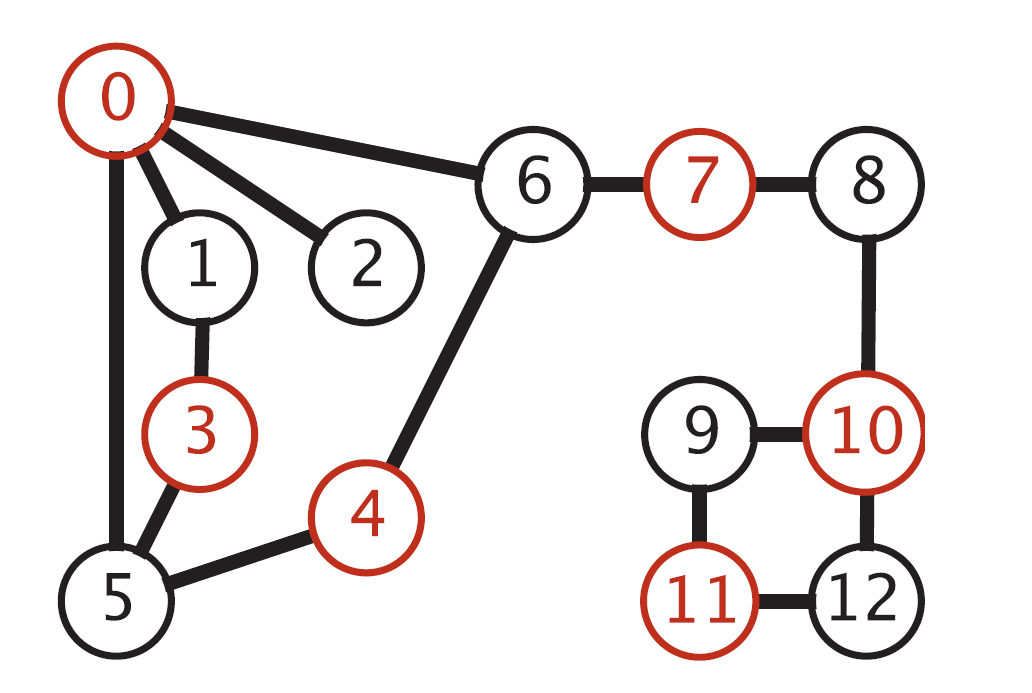
\includegraphics[scale=0.15]{img/graph_bipart.png}
	\caption{A bipartite graph}
	\label{fig:bipart}
\end{figure}

\subsubsection{Différents types de représentations des graphes}

Il y en a 3: 
\begin{itemize}
\item une liste de liens
\item une matrice d'adjascence
\item une liste d'adjascence 
\end{itemize}

Les complexités des méthodes \texttt{adj(int v)} et \texttt{addEdge(int v, int w)} sont les suivantes: 

\vspace{0.3cm}
\begin{tabular}{|c|c|c|c|}
\hline
& \textbf{Liste de liens} & \textbf{Matrice d'adjascence} & \textbf{Listes d'adjascence }\\
\hline
\textbf{adj(int v)} & O(m) & O(n) & O(1) 
\\
\textbf{addEdge(int v, int w)} & O(1) & O(1)& O(1)
\\
\hline
\end{tabular}

\subsubsection{DepthFirstSearch}



\lstinputlisting{code/DepthFirstSearch.java}

\subsubsection{DepthFirstPath}


\lstinputlisting{code/DepthFirstPath.java}


\begin{figure}[H]
	\centering
	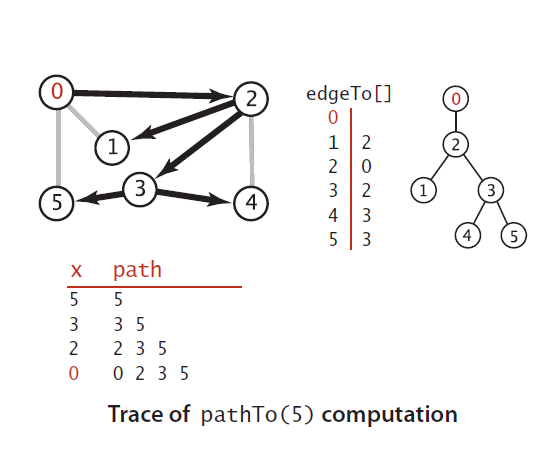
\includegraphics[scale=0.5]{img/dfp.png}
	\caption{Trace of pathTo(5) computation}
	\label{fig:dfp}
\end{figure}

\subsection{Graphes orientés}

\paragraph{Definition}

A directed graph (or digraph) is a set of vertices and a collection of directed
edges. Each directed edge connects an ordered pair of vertices.

\paragraph{Definition}

A directed path in a digraph is a sequence of vertices in which there is
a (directed) edge pointing from each vertex in the sequence to its successor in the
sequence. A directed cycle is a directed path with at least one edge whose first and
last vertices are the same. A simple cycle is a cycle with no repeated edges or vertices
(except the requisite repetition of the first and last vertices). The length of a path or
a cycle is its number of edges.

\subsubsection{DirectedDFS}

\lstinputlisting{code/DirectedDFS.java}

\subsubsection{DirectedCycle}

\paragraph{Definition}

A directed acyclic graph (DAG) is a digraph with no directed cycles.
\\

This class adds to our standard recursive dfs() a boolean array onStack[] to keep track of the vertices
for which the recursive call has not completed. When it finds an edge v->w to a vertex w that is on
the stack, it has discovered a directed cycle, which it can recover by following edgeTo[] links.

\lstinputlisting{code/DirectedCycle.java}

\begin{figure}[H]
	\centering
	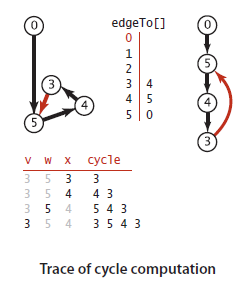
\includegraphics[scale=0.8]{img/directed_cycle.png}
	\caption{Trace of cycle computation	}
	\label{fig:directed cycle}
\end{figure}

\subsubsection{Tri topologique}

\paragraph{Proposition}
A digraph has a topological order if and only if it is a DAG.

Three vertex orderings are
of interest in typical applications:

\begin{itemize}
\item Preorder : Put the vertex on a queue before the recursive calls.
\item Postorder : Put the vertex on a queue after the recursive calls.
\item Reverse postorder : Put the vertex on a stack after the recursive calls.

\end{itemize}

\begin{figure}[H]
	\centering
	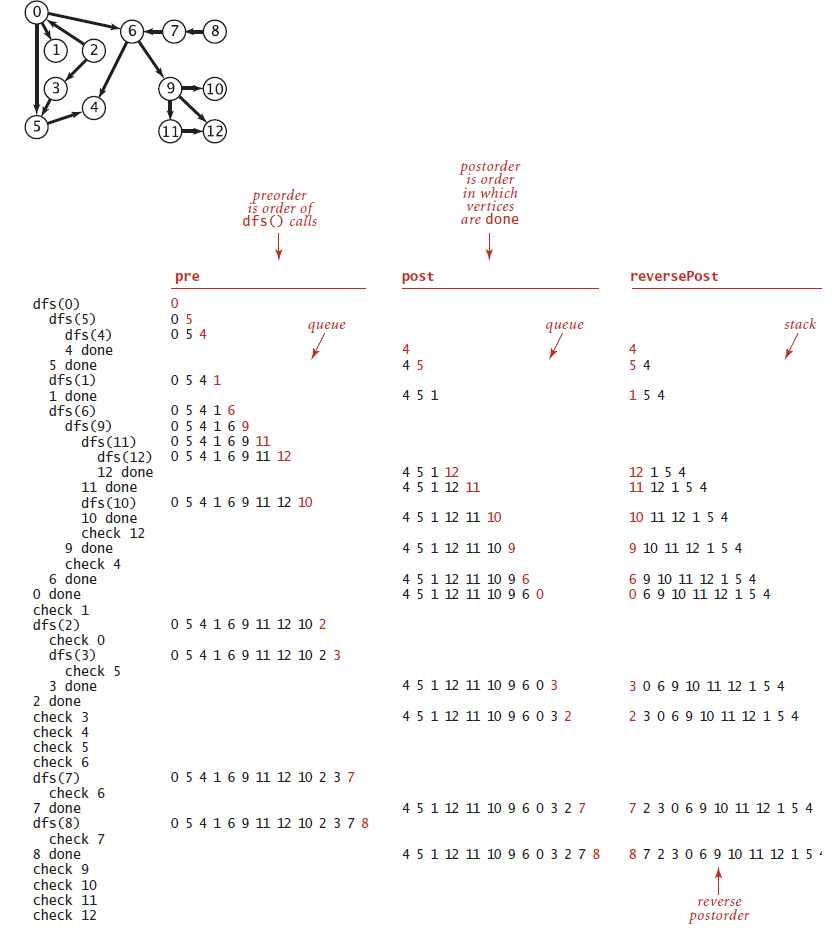
\includegraphics[scale=1]{img/pre_post_rev.png}
	\caption{Computing depth-first orders in a digraph}
	\label{fig:directed cycle}
\end{figure}



A
one-line addition to our standard recursive DFS does the job! To convince you of this
fact, we begin with the class DepthFirstOrder

\lstinputlisting{code/DFSOrder.java}

\lstinputlisting{code/TopologicalSort.java}

\subsection{Minimum Spanning Trees}

\paragraph{Definition}

A minimum spanning tree (MST ) of an
edge-weighted graph is a spanning tree whose weight
(the sum of the weights of its edges) is no larger than
the weight of any other spanning tree.

\paragraph{Definition}
A cut of a graph is a partition of its vertices into two nonempty disjoint
sets. A crossing edge of a cut is an edge that connects a vertex in one set with a vertex
in the other.

\paragraph{Edge-weighted graph data type}:

\begin{figure}[H]
	\centering
	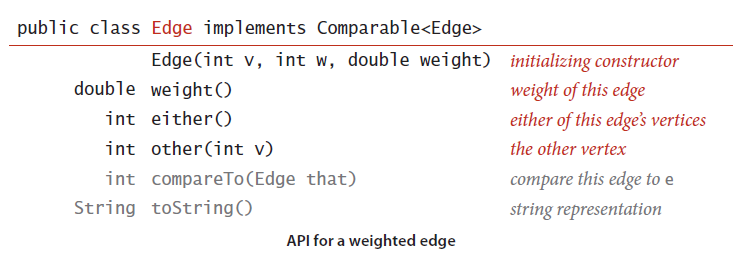
\includegraphics[scale=0.7]{img/edge_w_api.png}
	
	\label{fig:edge w api}
\end{figure}

\paragraph{Cut Property}

Given any cut in an edgeweighted
graph, the crossing edge of minimum weight is in
the MST of the graph.

\subsubsection{Prim's algorithm}

Prim’s algorithm computes the MST of any
connected edge-weighted graph.

\lstinputlisting{code/LazyPrimMST.java}

\subsubsection{Kruskal's algorithm}

\lstinputlisting{code/Kruskal2.java}

\subsubsection{Summary}

\begin{figure}[H]
	\centering
	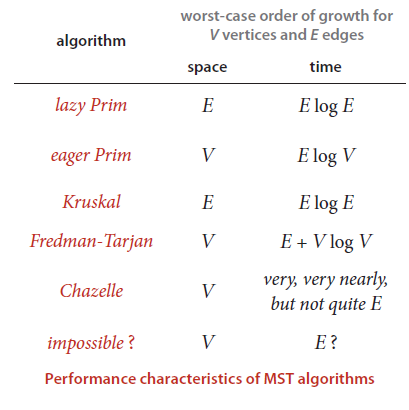
\includegraphics[scale=0.8]{img/summary_mst.png}
	
	\label{fig:summary MST}


\end{figure}


\subsection{Shortest path}

\begin{figure}[H]
	\centering
	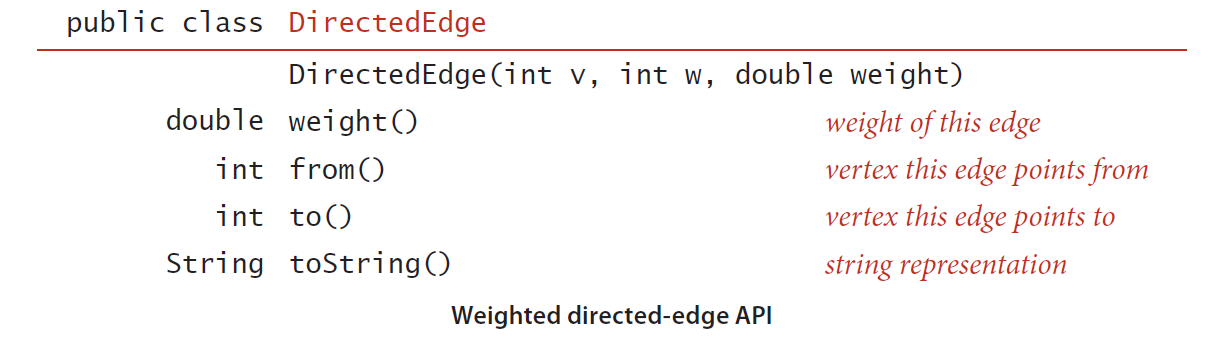
\includegraphics[scale=0.5]{img/directed_edge_w_api.png}
	
	\label{fig:directed w edge api}


\end{figure}


\subsubsection{Dijkstra's algorithm}
\lstinputlisting{code/Dijkstra.java}

\subsubsection{Summary}

\begin{figure}[H]
	\centering
	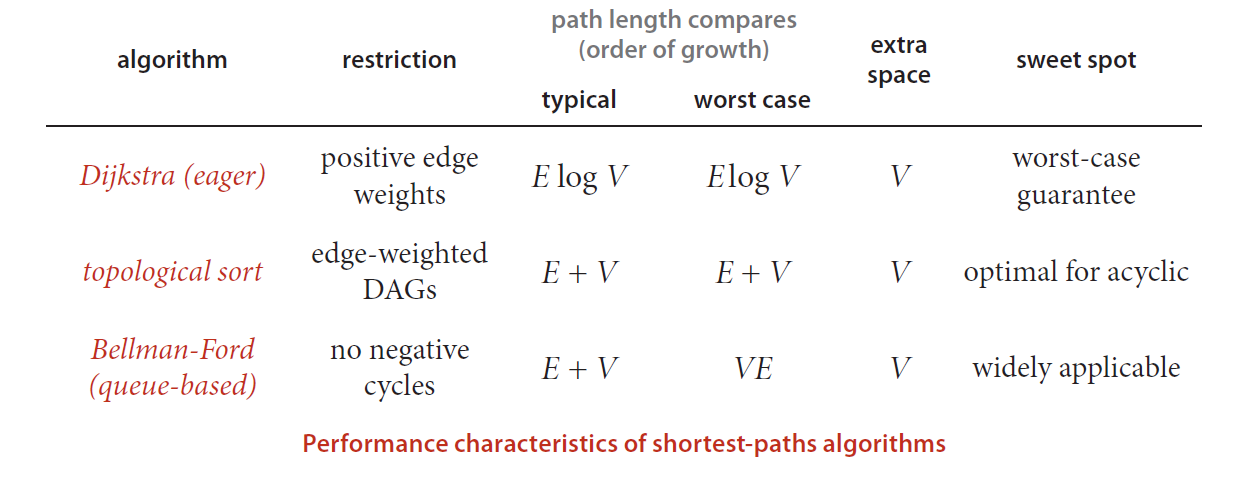
\includegraphics[scale=0.5]{img/summary_SPT.png}
	
	\label{fig:summary spt}


\end{figure}


% Need a better title for this section
\section{Various algorithms}
\subsection{Union-find}
\begin{mydef}
A \textit{union-find} data structure is a data structure
that keeps track of a set of elements partitionned into
a number of disjoint subsets (equivalence classes).
\end{mydef}

The API is given in figure \ref{fig:uf-api}.

\begin{figure}[ht]
	\centering
	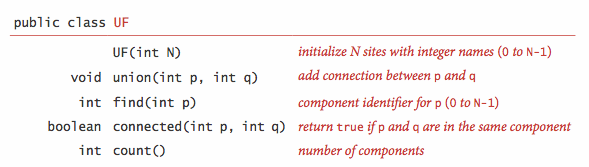
\includegraphics[scale=0.6]{img/uf-api.png}
	\caption{API of union-find data structure.}
	\label{fig:uf-api}
\end{figure}

This data structure helps to solve \textit{dynamic
connectivity} problem. This problem arises for example
in networks. We will use networking terminology here.
We refer to the objects as \textit{sites}, the paires
as \textit{connections} et equivalence classes as
\textit{connected components} or \textit{components}.

When studying algorithms to implement the union-find API,
we count array accesses (the number of times an array entry
is accessed, for read or write).

We will consider three different implementations, all based
on using a site-indexed \lstinline|id[]| array.

\subsubsection{Quick-find}
Here we maintain the invariant that \lstinline|p| and
\lstinline|q| are connected if and only if \lstinline|id[p]|
is equal to \lstinline|id[q]|. Implementation is quite
straightforward. An overview of quick-find is given
in figure \ref{fig:quick-find-overview}.

\begin{lstlisting}
public class UF {
	private int[] id;	// access to component id (site indexed)
	private int count;	// number of components
	
	public UF(int N) {
		count = N;
		id = new int[N];
		for(int i = 0; i < N; i++) {
			id[i] = i;		
		}	
	}
	
	public int count() { return count; }
	public boolean connected(int p, int q) { return find(p) == find(q);	}
	public int find(int p) {return id[p];}
	
	public void union(int p, int q) {
		int pID = find(p);
		int qID = find(q);
		
		if(pID == qID) return;
		
		for(int i = 0; i < id.length; i++)
			if(id[i] == pID) id[i] = qID;		
		
		count--;
	}
}
\end{lstlisting}

\begin{myrem}
Note that here we made the arbitrary choice of
renaming the component containing \lstinline|p|.
\end{myrem}

\begin{myprop}
The quick-find algorithm uses one array access for
each call to \lstinline|find()|, two array accesses
for each call to \lstinline|connected()| and
between $N+3$ and $2N+1$ array accesses for
each call to \lstinline|union()| that combines
two components.
\end{myprop}

\begin{figure}[ht]
	\centering
	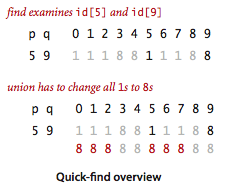
\includegraphics[scale=0.6]{img/quick-find-overview.png}
	\caption{Quick-find overview.}
	\label{fig:quick-find-overview}
\end{figure}

\subsubsection{Quick-union}
Here, the \lstinline|id[i]| entry for each site
is the name of another site in the same component
(possibly itself, in this case we call it a
\textit{root}) - we refer to this connection as a
\textit{link} To implement \lstinline|find()|,
we start at the given site, follow its link to
another site, follow that site's link to yet
another site and so forth until reaching a root.
An overview of quick-union is given
in figure \ref{fig:quick-union-overview}.

\begin{lstlisting}
public int find(int p) {
	while (p != id[p]) p = id[p];
	return p;
}
\end{lstlisting}

Two sites are in the same component if and
only if this process leads them to the same
root.

\begin{lstlisting}
public void union(int p, int q) {
	int i = find(p);
	int i = find(q);
	if (i == j) return;
	
	// Make root of the first tree point to the second
	id[i] = j;
	count--;
}
\end{lstlisting}

\begin{figure}[ht]
	\centering
	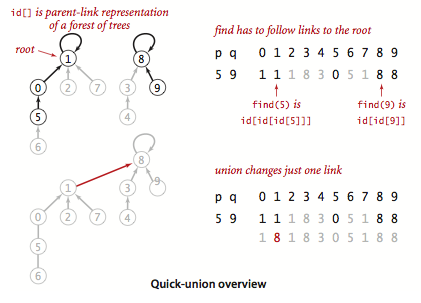
\includegraphics[scale=0.55]{img/quick-union-overview.png}
	\caption{Quick-union overview}
	\label{fig:quick-union-overview}
\end{figure}

On figure \ref{fig:quick-union-overview}, we use the
\textit{forest-of-trees} representation. With this
representation, we can define some terminology.

\begin{mydef}
The \textit{size} of a tree is its number of notes. The
\textit{depth} of a node in a tree is the number of links on the
path from it to the root. The \textit{height} of a tree is
the maximum depth among its nodes.
\end{mydef}

\begin{myprop}
The number of array accesses used by \lstinline|find()| in
quick-union is 1 plus twice the depth of the node corresponding
to the given site. The number of array accessed used by
\lstinline|union()| and \lstinline|connected()| is the cost
of the two \lstinline|find()| operations (plus 1 for \lstinline|union()|
if the given sites are in different trees).
\end{myprop}

\subsubsection{Weighted-quick-union}
Weighted-quick-union is an improvement to quick-union algorithms
that allow us to reduce the tree height, and thus to reduce
complexity of \lstinline|find()|.

\begin{lstlisting}
public class WeigthedQuickUnionUF {
	private int[] id;	// access to component id (site indexed)
	private int[] sz;	// size of component for roots (site indexed)
	private int count;	// number of components
	
	public WeightedQuickUnionUF(int N) {
		count = N;
		id = new int[N];
		for(int i = 0; i < N; i++)	id[i] = i;
		sz = new int[N];		
		for(int i = 	0; i < N; i++) 	sz[i} = 1;	
	}
	
	public int count() { return count; }
	public boolean connected(int p, int q) { return find(p) == find(q);	}
	
	public int find(int p) {
		while(p != id[p]) p = id[p];
		return p;
	}
	
	public void union(int p, int q) {
		int i = find(p);
		int j = find(q);
		if(i == j) return;
		
		// Make smaller root point to the larger one
		if		(sz[i] < sz[j]) 	{ id[i] = j; sz[j] += sz[i]; }
		else						{ id[j] = i; sz[i] += sz[j]; }
		
		count--;
	}
}
\end{lstlisting}

\begin{myprop}
The depth of any node in a forest built by weighted
quick-union for $N$ sites is at most $\log N$.
\end{myprop}

\begin{mycorr}
For weighted quick-union with $N$ sites, the worst
case order of growth of the cost of \lstinline|find()|,
\lstinline|connected()| and \lstinline|union()| is
$\log N$.
\end{mycorr}

\subsubsection{Summary}

\begin{table}[ht]
	\centering
	\begin{tabular}{c|ccc}
		\textbf{algorithm} & \textbf{constructor} & \textbf{union} & \textbf{find} \\
		\hline
		quick-find & $N$ & $N$ & 1 \\
		quick-union & $N$ & tree height & tree height \\
		weigthed quick-union & $N$ & $\log N$ & $\log N$
	\end{tabular}
	\caption{Performance characteristics of union-find algorithms.}
	\label{tab:perf-uf}
\end{table}

\subsection{Priority queues}
A priority queue is an abstract data type with the API given
in figure \ref{fig:pq-api}. In this subsection, we will
consider a \lstinline|MaxPQ|. \lstinline|MinPQ| is easily
obtained from \lstinline|MaxPQ| (you only need to use
min-heap instead of a max-heap, continue to read to understand).

\begin{figure}[ht]
	\centering
	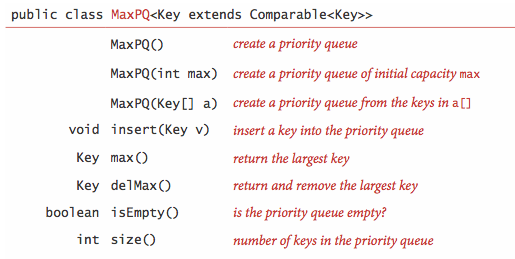
\includegraphics[scale=0.55]{img/pq-api.png}
	\caption{API of a priority queue.}
	\label{fig:pq-api}
\end{figure}

\subsubsection{Basic implementations}
Basic implementations using (un)ordered arrays or linked
list have the property that either the insert of the remove
maximum operation takes linear time in the worst case.

\subsubsection{Heap}
The binary heap is a data structure that can efficiently support
the basic priority queues operations. In a binary heap, the keys
are stored in an array such that each key is guaranteed to be
larger than (or equal to) the keys at two
other specific positions.

\begin{mydef}
A binary tree is \textit{heap-ordered} if the key in each
node is larger than or equal to the keys in that node's
two children (if any).
\end{mydef}

\begin{myprop}
The largest key in a heap-ordered binary tree is found at
the root.
\end{myprop}

\begin{mydef}[Complete binary tree]
In a complete binary tree every level, except possibly the
last, is completely filled, and all nodes in the last level
are as far left as possible.
\end{mydef}

A heap-ordered complete binary tree is illustrated in figure
\ref{fig:heap}.

\begin{figure}[ht]
	\centering
	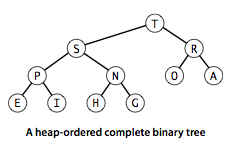
\includegraphics[scale=0.55]{img/heap.png}
	\caption{A heap-ordered complete binary tree.}
	\label{fig:heap}
\end{figure} 

Complete trees provide the opportunity to use a compact
array representation (instead of explicit links as
for trees of section \ref{sec:tree}).

\begin{mydef}
A binary heap is a collection of keys arranged in a complete
heap-ordered binary tree, represented in level order in an
array (not using the first entry).
\end{mydef}

In a heap, the parent of the node in position $k$ is in
position $\lfloor \frac{k}{2} \rfloor$ and, conversely,
the two children of the node in position $k$ are in
position $2k$ and $2k+1$. This allows us to travel
up and down the tree simply by doing arithmetic on
on array indices.

\begin{myprop}
The height of a complete binary tree of size $N$ is
$\lfloor \log N \rfloor$
\end{myprop}

\paragraph{Heap algorithms}
Operations on heap could violate the heap condition.
The process of restoring the heap order is called
\textit{reheapifying}. There is two types of violation
and thus two algorithms ro reheapify.

\subparagraph{Bottom-up reheapify (swim)}
If the heap order is violated because a node's key become
larger than that node's parent's key, then we can make
progress toward fixing the violation by exchanging the node
with its parent (and so forth, moving up until we reach a
node with a larger key, or the root).

\begin{lstlisting}
private void swim(int k) {
	while(k > 1 && less(k/2, k)) {
		exch(k/2, k);
		k = k/2;	
	}
}
\end{lstlisting}

\subparagraph{Top-down reheapify (sink)}
If the heap order is violated because a node's key
becomes smaller than one or both of that children's
key, then we can make progress toward fixing the
violation by exchanging the node with the larger
of its two children (and so forth, moving down until
we reach a node with both children smaller (or equal),
or the bottom).

\begin{lstlisting}
private void sink(int k) {
	while(2*k <= N) {
		int j = 2*k;
		// Make j point to the larger of the two children
		if(j < N && less(j, j+1)) j++;	
		if(!less(k, j)) break;
		exch(k, j);
		k = j;	
	}
}
\end{lstlisting}


\begin{figure}[ht]
	\centering
	\begin{subfigure}{.5\textwidth}
		\centering
  		\includegraphics[width=.85\linewidth]{img/swim.png}
 		\caption{Swim.}
  		\label{fig:siwm}
	\end{subfigure}%
	\begin{subfigure}{.5\textwidth}
  		\centering
  		\includegraphics[width=0.73\linewidth]{img/sink.png}
  		\caption{Sink.}
  		\label{fig:sink}
	\end{subfigure}
	\caption{}
	\label{fig:reheap}
\end{figure}

\paragraph{Implementations}
Now that we can reheapify, implementing \lstinline|MaxPQ|
is quite straightforward.

\begin{lstlisting}
public class MaxPQ<Key extends Comparable<Key>> {
	private Key[] pq;
	private int N = 0;
	
	public MaxPQ(int maxN) {
		pq = (Key[]) new Comparable[maxN+1];	
	}
	
	public boolean isEmpty() { return N == 0; }
	public int size() { return N; }
	
	public void insert(Key v) {
		pq[++N] = v;
		swim(N);
	}
	
	public Key delMax() {
		Key max = pq[1];
		exch(1, N--);
		pq[N+1] = null;
		sink(1);
		return max;	
	}
}
\end{lstlisting}

Heap operations are illustrated in figure \ref{fig:heap-ops}.

\begin{figure}[ht]
	\centering
	\includegraphics[scale=0.55]{img/heap-ops.png}
	\caption{Heap operations.}
	\label{fig:heap-ops}
\end{figure} 

\begin{myprop}
In a $N$-key priority queue, the heap algorithms
require no more than $1 + \log N$ compares for
insert and no more than $2\log N$ compares
for remove the maximum.
\end{myprop}

\end{document}
